%                                                                 aa.dem
% AA vers. 9.1, LaTeX class for Astronomy & Astrophysics
% demonstration file
%                                                       (c) EDP Sciences
%-----------------------------------------------------------------------
%
% \documentclass[referee]{aa} % for a referee version
%\documentclass[onecolumn]{aa} % for a paper on 1 column  
%\documentclass[longauth]{aa} % for the long lists of affiliations 
% \documentclass[letter]{aa} % for the letters 
%\documentclass[bibyear]{aa} % if the references are not structured 
%                              according to the author-year natbib style

%
\documentclass{aa}  

%
\usepackage{amsmath}
\usepackage{graphicx, comment}
\usepackage{commath}
\usepackage{txfonts}
\usepackage{subfig}
\usepackage{upgreek}
\usepackage{threeparttable} 
\usepackage{booktabs}
\usepackage{siunitx}
\usepackage{natbib}
\usepackage{float}
\usepackage{enumitem}

% \usepackage[backend=biber, style=authoryear, natbib=true]{biblatex}
% 超链接配置：确保链接颜色可见，去除边框
\usepackage[colorlinks=true, linkcolor=blue, urlcolor=blue, citecolor=blue]{hyperref}
\usepackage{orcidlink}

\newcommand{\C}{3C\,84}
\newcommand{\rotang}{-4.5^\circ}
\newcommand{\protang}{4.5^\circ}
\newcommand{\beam}{(0.17\times0.40)\,\textrm{mas}}

\newcommand{\Mj}{5.0\pm1.7}
\newcommand{\Mjrel}{6.7\pm2.0}
\newcommand{\Mx}{9.8\pm3.2}
\newcommand{\enthalpy}{0.26\pm0.20}
\newcommand{\ajj}{0.14\pm0.06}
\newcommand{\ax}{0.07\pm0.02}
\newcommand{\bw}{0.27\pm0.04}

\newcommand{\rj}{0.36\pm0.09\,\textrm{pc}}
\newcommand{\phij}{4.5^\circ\pm1.2^\circ}
\newcommand{\thetaj}{35^\circ\pm5^\circ}
\newcommand{\gj}{1.35\pm0.14}


\newcommand{\tp}{30\pm10\,\textrm{years}}
\newcommand{\chiamp}{\sim1}
\newcommand{\chialt}{\sim2}




\begin{document} 

\renewcommand{\arraystretch}{1.5}
   
    \title{
    % 1.4GHz下对低红移射电星系的统计：用多种视角观察射电星系的特性
    Morphology Statistics of the Fanaroff-Riley I and II Sources
    }

    \author{
        P.-G. Zheng\inst{1,2}
    \and R.-Y. Ma\inst{1,2}\thanks{Corresponding author: \email{ryma@xmu.edu.cn}}
    \and Z.-H. Zhu\inst{3,2}\thanks{Corresponding author: \email{}}
    \and X. Cao\inst{1,2}
    \and Y. Xie\inst{4}\thanks{Corresponding author: \email{xieyi@jmu.edu.cn}}
    \and X.-L. Wang\inst{1,2}
    }
    
    \institute{
    Department of Astronomy and Institute of Theoretical Physics and Astrophysics, Xiamen University, Xiamen, Fujian 361005, China
    \and
    SHAO--XMU Joint Center for Astrophysics, Xiamen, Fujian 361005, China
    \and
    Shanghai Astronomical Observatory, Chinese Academy of Sciences, 80 Nandan Road, Shanghai 200030, China
    \and
    School of Science, Jimei University, Xiamen 361021, Fujian Province, China
    }




   \date{Received -; accepted -}


 \abstract
   {
   Jet lobes of Radio Galaxies (RGs) are vital components shaped primarily by interactions with the circumgalactic medium. This study focuses on extracting morphological parameters of Fanaroff-Riley (FR)\textemdash classified RGs (FRI and FRII) from 1.4 GHz radio images via elliptical structure fitting, aiming to systematically characterize their morphological properties. A semi-automated workflow is developed to localize the RG cores and lobes. 
    Our key results are as follows:
    (1) We performed a systematic statistical analysis of RG morphological properties, adopting the aspect ratio as the primary metric to quantify their structural signatures. Using this framework, we statistically verified the intrinsic physical differences between FRI and FRII populations, and suggest a correlation between the double-lobe brightness ratio and the positional offset ratio of their optical counterparts within the aspect ratio range of [0.2, 0.3].
    (2) We applied the classical $r_s$ method to our full sample, and uncovered a prominent, parameter-insensitive substructure in FRIIs at $r_s$<0.3. This feature is robust against variations in algorithm tuning, which remains stable across different algorithm tuning configurations.
    (2) Via the classical $r_s$ method for sample analysis, and detect a distinct, parameter-insensitive substructure for FRIIs at $r_s$<0.3, which remains stable across different algorithm tuning configurations.
    (3) We perform knot enumeration using a flood-filling approach with a maximum brightness threshold to track the evolutionary characteristics of knot structures, with cross-validation confirming that these knots are not induced by random flux fluctuations.
    (4) We construct the central line of RGs and reveal the average radiatively active regions of RGs via brightness stacking of central lines from a sufficiently large sample.
    Collectively, our multi-perspective analysis clarifies the structural properties and evolutionary mechanisms of FR-classified RGs, and refines the existing understanding of FR morphological classification. In this study, we combine well-established methodologies from prior literature with our novel technical approaches to conduct a comprehensive characterization of FRIs and FRIIs from the Faint Images of the Radio Sky at Twenty-Centimeters (FIRST) survey.
    
   }
 
  

   \keywords{
            Active galactic nuclei; Radio galaxy; Radio astronomy
               }

   \maketitle

   
\section{Introduction}\label{sec:Introduction}
% 介绍RGs重要性
Radio galaxies (RGs) are a class of active galaxies whose prominent radio emission is powered by relativistic jets launched from the central supermassive black hole. Their radio structures span an enormous range of spatial scales, from parsecs to megaparsecs \citep{hardcastle_radio_2020}. It is now well established that luminous RGs play key roles in regulating galaxy evolution and the formation of cosmic large-scale structures \citep{miley_distant_2008}. The general picture of RGs has been widely accepted: the central black hole powers the jet with rotational energy extracted either from the black hole itself via the Blandford–Znajek process or from the accretion flow via the Blandford–Payne process \citep{BZ77,BP82}; the energy is then transferred outward along large-scale magnetic fields, accompanied by the acceleration of bulk motion and relativistic particles. At the jet–ambient medium interface, the external intergalactic medium plays a crucial role in shaping the morphology of the extended radio structure \citep[e.g.,][and references therein]{BlandfordRees1978,ghisellini_bulk_1989,blandford_relativistic_2019}.

Observationally, RGs have been classified in multiple complementary ways according to their morphology, spectral index, emission-line properties, and radio-to-optical flux ratio \citep[e.g.,][]{fanaroff_morphology_1974,osterbrock_broad_1975,heckman_optical_1980,veilleux_spectral_1987,owen_ccd_1989,kellermann_radio_1989}. Among these, the most widely adopted and historically earliest morphological classification is the Fanaroff–Riley (FR) scheme, proposed by \citet{fanaroff_morphology_1974}. This scheme divides extended radio sources into two types based on the ratio 
of the separation between the brightest regions on the two lobes to the total linear size of the radio structure. FRI sources are centre-brightened, with surface brightness decreasing from the core outward along symmetric large-scale jets, and are typically less luminous. FRII sources are edge-brightened, with bright hot spots near the outer extremities of more collimated, often asymmetric jets, and are typically more luminous \citep{ledlow_20cm_1996}.

Subsequent studies have demonstrated that radio luminosity alone is not a reliable indicator for determining FR type: sources with identical radio luminosity can display either FRI or FRII morphology \citep[e.g.,][]{mingo_revisiting_2019}. \citet{ledlow_20cm_1996} found that the FRI/FRII dividing line in the radio-luminosity–optical-magnitude plane is not sharp but rather a function of the host galaxy's optical luminosity, with brighter host galaxies requiring higher radio luminosities for the FRI-to-FRII transition. \cite{lin_populations_2010} further proposed using the ratio as a quantitative diagnostic parameter to discriminate between RGs of different morphologies. A particularly intriguing subset is the hybrid morphology radio sources (HYMORS), first identified by \citet{gopal-krishna_extragalactic_2000}, in which one lobe exhibits FRI structure while the opposite lobe shows FRII structure — a phenomenon that provides strong constraints on theoretical models for the FR dichotomy. 

The physical origin of the FRI/FRII dichotomy has attracted intense theoretical interest. Explanations generally fall into three categories: those invoking intrinsic differences in the central engine \citep[e.g.,][]{Baum1995,Meier1999,hardcastle_radio_2020}, such as black hole spin, accretion mode, or jet composition; those attributing the dichotomy to the external environment, including the location where the initially supersonic jet decelerates or encounters a density jump in the ambient medium \citep[e.g.,][]{de_young_relation_1993,bicknell_relativistic_1995,bowman_deceleration_1996,liu_environment_2019}; and those focusing on the jet itself, such as its initial power and stability \citep[e.g.,][]{florido_spatial_1990,Reynolds1996,Meier1997,lane_3c_2002}. The existence of HYMORS argues strongly against explanations that rely solely on central-engine properties — a single black hole is unlikely to produce jets of fundamentally different natures in opposite directions simultaneously \citep{gopal-krishna_extragalactic_2000} — and instead favors models in which the FR morphology is primarily determined by the jet–environment interaction. This conclusion is further supported by recent relativistic magneto-hydrodynamic simulations, which demonstrate that the plasma properties of the jet --- specifically, the composition (electron--positron versus electron--proton) and the magnetization --- critically determine whether the resulting large-scale morphology resembles an FRI or FRII source \citep{tripathi_how_2026}.
Despite these ongoing debates, the FR classification remains the foundational taxonomic scheme for extended radio galaxy studies \citep[e.g.,][]{kapinska_lofar_2017,capetti_friicat_2017a,capetti_friicat_2017b,saikia_radio_2022}.

The morphological studies of RGs are helpful in many aspects. 
On the one hand, the morphology imprints the ancient activities of the host galaxies, such as mergers and recurrent episodes of AGN activity \citep[e.g.,][]{merritt_tracing_2002,liu_x-shaped_2004,hardcastle_ngc_2019,lara_restarting_1999,saikia_recurrent_2009,kuzmicz_optical_2017}. On the other hand, the morphology is a consequence of the interaction between jets and the environmental medium, which can be used to estimate the effects of feedback \citep{begelman_theory_1984,blandford_relativistic_2019}. Moreover, a better understanding of RGs will facilitate subtraction of the foreground extragalactic contamination to the 21 cm line of neutral hydrogen emitted during the epoch of reionization \citep{di_matteo_radio_2002,di_matteo_21-cm_2004}, and is therefore meaningful for understanding cosmic evolution \citep{madau_21_1997,tozzi_radio_2000,furlanetto_cosmology_2006}.

In recent years, more extensive and quantitatively detailed morphological studies of RGs have been conducted. 
\cite{lin_populations_2010} statistically investigated how various physical properties are correlated with the FRI/FRII morphological classification. \cite{mingo_revisiting_2019} developed an automated morphological classification tool based on quantitative physical properties. 
The propagation direction of the jets, or the ridge lines, has been reconstructed by tracing the peaks of flux densities in radio jets \citep[e.g.,][]{barkus_application_2021,velovic_collimation_2022,clews_radio-loud_2025}. \cite{park_discovery_2024,foschi_evolution_2025} extracted the spine--sheath structure from transverse profiles to investigate limb-brightened jet morphology. However, the morphological features of RGs still merit further investigation to uncover the physics underlying their formation mechanisms.
However, the morphological features of RGs are still worthy of  further quantitative investigations to uncover the differences between different types of radio sources.
Based on the above methodological advancements in RG morphological characterization, as well as new survey of radio sky, in this work we  model the morphology of the radio galaxies with an ellipse and a cental line,  which could show the interaction between the kinetic energy of the jet and the intergalactic medium to some extent, not only along the jet direction but also along the  vertical direction. And then we statistically investigate the distribution of quantitative parameters..
As the first step, we concentrate only on the well defined FRIs and FRIIs. 
The FR0 sources are not included as observations of high spatial resolution are needed. The hybrid sources are also ignored, as the number of such sources are quite limited. 


This paper is organized as follows. Section \ref{sec:Data} introduces the datasets utilized. Section \ref{sec:Method} describes the method and the geometric parameters. Section \ref{sec:Result} presents the results, and discussion are made in Section \ref{sec:Discussion}. Finally, summary and future researches are listed in Section \ref{sec:Conclusions and Future}.
For this paper, we have used a Lambda cold dark matter ($ \Lambda\text{CDM} $) cosmology model for the Universe with Hubble constant $H_{0}$ = 67.74 km/s/Mpc, $\Omega_m$ = 0.3089 and $\Omega_\Lambda$ = 0.6911 based on Planck measurements \citep{collaboration_planck_2016}.



\section{Data}\label{sec:Data}
The original dataset comes from the Faint Images of the Radio Sky at Twenty-centimeters (FIRST), 
which produced the radio equivalent of the Palomar Observatory Sky Survey over 10,000 square degrees of the North and South Galactic Caps.
Using the NRAO Very Large Array (VLA) and an automated mapping pipeline, images with 1.8\arcsec pixels, a typical rms of 0.15 mJy, and a resolution of 5\arcsec are obtained.
And at the 1 mJy source detection threshold, there are $\sim$90 sources per square degree, $\sim$35\% of which have resolved structure \textcolor{red}{on scales from 2-30\arcsec. }
About 30\% of the sources \textcolor{red}{have counterparts in the Sloan Digital Sky Survey (are in the region that have been covered by the SDSS?)}\footnote{\url{https://sundog.stsci.edu/}}. 
\cite{griese_first_2023} processed the datasets with denoising and cropping\textemdash to ensure data quality\footnote{\url{https://github.com/floriangriese/RadioGalaxyDataset}},
and 2,158 images in total with 495 FRIs, 924 FRIIs, 391 compact sources, and 348 bent sources, are derived \citep{griese_floriangrieseradiogalaxydataset_2022}. 
\textcolor{red}{As a first step, we excluded those sources with complex structure.}

\textcolor{red}{For most sources, the host galaxies have been identified in previous works, and we therefore adopted their results},
which could be obtained by conducting queries via the VizieR\footnote{\url{https://vizier.cds.unistra.fr/}} astronomical data service.
\textcolor{red}{For those sources, of which the host galaxies have not been identified, we match the .... }.
Considering the pixel scale of the FIRST telescope snapshot images, and the fact that the selected central position might be offset within the surrounding pixel region, the search radius of 5\arcsec was adopted. 
According to the NASA/IPAC Extragalactic Database (NED)\footnote{\url{https://ned.ipac.caltech.edu/}}, possible optical counterparts of the host galaxies are therefore found. 
\textcolor{red}{If there are more than one sources, we select the closest ... } 
Our method agrees well with previous works.
\textcolor{red}{Generally,  the host galaxies of  ... sources are identified}.

On  the one hand, the host galaxies are therefore used as the origin of the radio structure in following analysis.
On the other hand,  the information of the host galaxies can be retrieved from literature, such as redshift, stellar mass, central black hole mass.  It should be noted that the information of host galaxies maybe different for different catalogs. In this case, the averaged value is adopted for simplicity. 

For the radio sources with imaging data, previous studies have identified host galaxies for 167 FRI and 498 FRII sources. Of these hosts, central black hole masses have been estimated for 101 FRIs and 217 FRIIs, while stellar masses are available for 147 FRIs and 192 FRIIs.

The number distribution of the sources over redshift, central black hole mass and stellar mass are shown in Figure \ref{fig:Redshift&MassDistribution}. 
It can be seen that the redshifts of FRIs are lower than those of FRIIs. This should be selection effects as FRIIs are more powerful and therefore can be seen from farther place.
The distributions of black hole mass and stellar mass are broadly similar between FRIs and FRIIs, both in range and peak values.



\section{Method}\label{sec:Method}

In this work, we characterize radio morphologies by fitting ellipses that nearly fully enclose the radio-emitting structure. The ellipticity, quantified as the axial ratio of the semi-major to semi-minor axis, serves as a quantitative proxy for the interplay between jet propagation along the primary direction and lateral expansion perpendicular to it, and has been used in previous analyses of RG structure \citep[e.g.,][]{lin_new_2024, carilli_cygnus_1996, begelman_overpressured_1989}.
We further employ image processing techniques to trace the trajectory of the jet spine, which we refer to as the centerline. The intensity profile extracted along this centerline reveals how the jet evolves along its propagation axis as it interacts with the ambient medium. Together, the fitted ellipse and the extracted centerline offer a more comprehensive and quantitative description of the radio structure.
Starting from preprocessed images, we apply a sequence of image processing methods including flood-filling, Principal Component Analysis, and skeletonization to derive both the best-fitting ellipse and the centerline of the radio source. The detailed procedure is outlined below.



To further suppress background noise and eliminate contamination from complex low-surfac  e-brightness regions, we retain only pixels whose intensity exceeds a defined threshold. The threshold is set at the 95th percentile of the maximum brightness. We tested threshold values ranging from 50\% to 95\% and found that the results are insensitive to this choice. Once the threshold is chosen, we extract the connected above-threshold radio-emitting region via a flood-filling algorithm \citep[e.g.,][]{mingo_revisiting_2019,hales_blobcat_2012}.

Two physically unrelated radio sources may appear in close angular proximity due to projection effects, making it necessary to identify and exclude contamination that projection may introduce. Principal Component Analysis provides a natural framework for this task: it discards noise and fluctuations while drastically reducing the dimensionality of the image vector \citep[e.g., PCA tomography][]{hofmann_kernel_2008，steiner_pca_2009}. The first principal axis corresponds to the dominant orientation of the emission. Foreground or background sources, typically much smaller in angular extent than the target source, may perturb this principal direction, but the resulting deviation is generally minor. Moreover, such interlopers tend to be offset from the host galaxy position relative to the principal axis and can therefore be effectively filtered out. Intervening sources that happen to lie along the principal axis cannot be excluded in this way, yet their small sizes and low numbers mean they introduce negligible bias to the final result.

Once the filtered radio-emitting region is obtained, we describe it with a single ellipse. Two competing objectives guide the ellipse fitting: maximizing the fraction of the radio-emitting area covered by the ellipse, and minimizing the fraction of the ellipse interior that is non-emitting, so that the ellipse tightly hugs the radio lobes. For each candidate ellipse, \textcolor{red}{ we compute the uncovered radio-emitting area fraction and the non-emitting area fraction within the ellipse. The ellipse that minimizes the sum of these two fractions is selected as the final representation----}.

For the extracted radio-emitting region, we further apply skeletonization to obtain a one-pixel-wide, topologically faithful representation of the radio structure, which we define as the centerline \cite{vardoulaki_fr-type_2021}. Skeletonization achieves substantial data compression while preserving the essential topology of the image. We then employ a Breadth-First Search algorithm, constrained by the host galaxy position and the principal axis derived from PCA, to identify the most representative primary backbone of the skeleton. Conceptually, skeletonization resembles the ridge-line method used to finely trace continuous radio structures \cite{barkus_application_2021}; however, the ridge-line approach becomes problematic for larger-scale sources that exhibit discontinuities or significant curvature, where skeletonization remains robust.

\autoref{fig:Figure2} specifically presents the fitted ellipses and central lines for example radio galaxies, the coordinates (R.A. , Dec.) of which are as follows: (149.318°, 19.114°), (150.738°, 19.865°), (175.545°, 55.458°), (180.424°, 22.946°), (213.728°, 22.633°), (125.391°, 47.043°).


% 大概介绍一下目的（结论），以及用这些方法能得到什么
% 在这里介绍\cite{lin_populations_2010}是否合适？
%In the subsequent semi-automated workflow of this study, multiple processing methods for RGs are integrated. The core objective of this workflow is to obtain a general structural description\textemdash elliptical models\textemdash for FR-type RGs; and, the intermediate results derived from each step of the workflow are also worthy of discussion: Utilizing the flood-filling algorithm, brightness contours of RGs under specified brightness thresholds can be extracted; in particular, adjusting the brightness threshold to obtain the corresponding contours for FRIs allows us to uncover the evolutionary characteristics of their clumpy structures. The parameter $r_s$ proposed by \cite{lin_populations_2010}, serves as a classic criterion for FR-type classification; in the present study, the elliptical Gaussian model is utilized for the extracting $r_s$ of FRII galaxies. The central line defined in this study introduces a novel approach to describing the brightness distribution in the central regions of RGs; stacking the central line brightness distributions of FRII populations reveals prominent radiation-active regions, which is consistent with theoretical predictions. Additionally, the Principal Component Analysis (PCA) algorithm facilitates the derivation of the elongation parameter for RGs; owing to its straightforward processing approach, elongation parameter unexpectedly provides a quantitative measure for comparing the structural similarities between FRIs and FRIIs.

%\subsection{Semi-Automated Workflow}\label{sec:Section3_1}

% 自动化方法很重要
%Following an extensive literature review, \cite{mingo_revisiting_2019} highlighted the necessity of automated approaches for the scientific analysis of datasets from modern radio surveys. \cite{gupta_machine_2025} had similarly conducted work on the automated analysis of data from radio surveys. While automated algorithms excel at classifying compact, unresolved objects, extended sources remain a key challenge \citep{boyce_hydra_2023,boyce_hydra_2023-1}. Integrating multiple methodologies to conduct semi-automated analysis of extended sources is thus imperative.

%    The first step, this work will utilize the preclassified sample set from the \cite{griese_floriangrieseradiogalaxydataset_2022}, relevant information about which has been described in \autoref{sec:Data}. Herein, the use of standard cosmological models is required for the conversion of luminosity and physical scale. Given that the image data employed in this work have undergone brightness normalization (scaled to the range 0–255), it is further necessary to retrieve the flux densities of FRIIs to convert pixel brightness into physically meaningful flux values. By querying the specified FRIIs in the FIRST catalog via VizieR and combining this with previously collected information, an inverse transformation of the method presented in \cite{griese_first_2023} can be performed, thereby enabling us to compute the required physical quantities.
    

%The data acquired in \autoref{sec:Data} exhibit certain imperfections, most notably some RGs with extremely low overall brightness: all bright sources in the image appear extremely faint, or extremely bright ones interfere with target RGs' structure. Such images thus need exclusion from the dataset.

% Reliable reference structures differ across morphological classes: FRIs exhibit well-defined bright cores, whereas only hotspots in FRII systems show consistent detectability. Here, elliptical Gaussian models are fitted to sequentially decompose Gaussian components within the RG system. Despite the distinct structural characteristics of the two FR classes, a minimal ellipse that optimally encloses the entire RG can still be identified. This procedure also extracts the geometric parameters and physical properties of the radio galaxies.

%\begin{figure*}[!htbp]
%    \centering
%    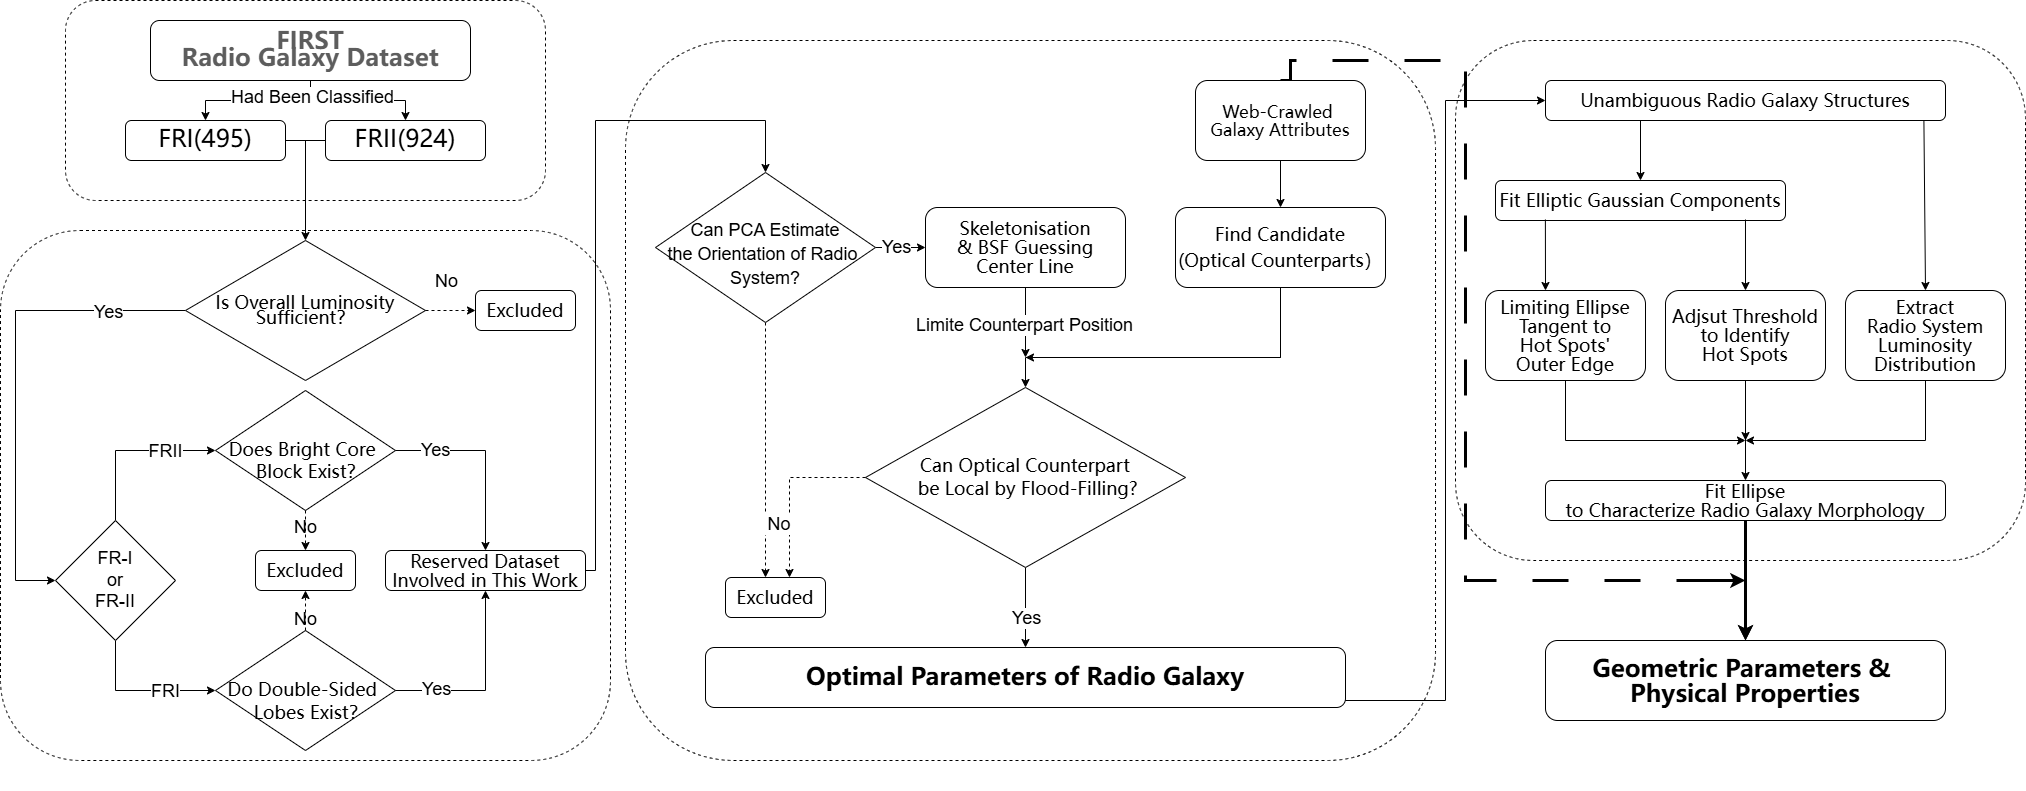
\includegraphics[width=0.9\linewidth]{Figure/Section 3/FR_type_operate.drawio.png}
%    \caption{Flowchart for processing FR-classified RGs in \autoref{sec:Method}. The ultimate goal of this job is to conduct statistics on the relevant parameters of the RG.}
%    \label{fig:FR_type_operate}
%\end{figure*}


\begin{figure}[!htbp]
    \centering
    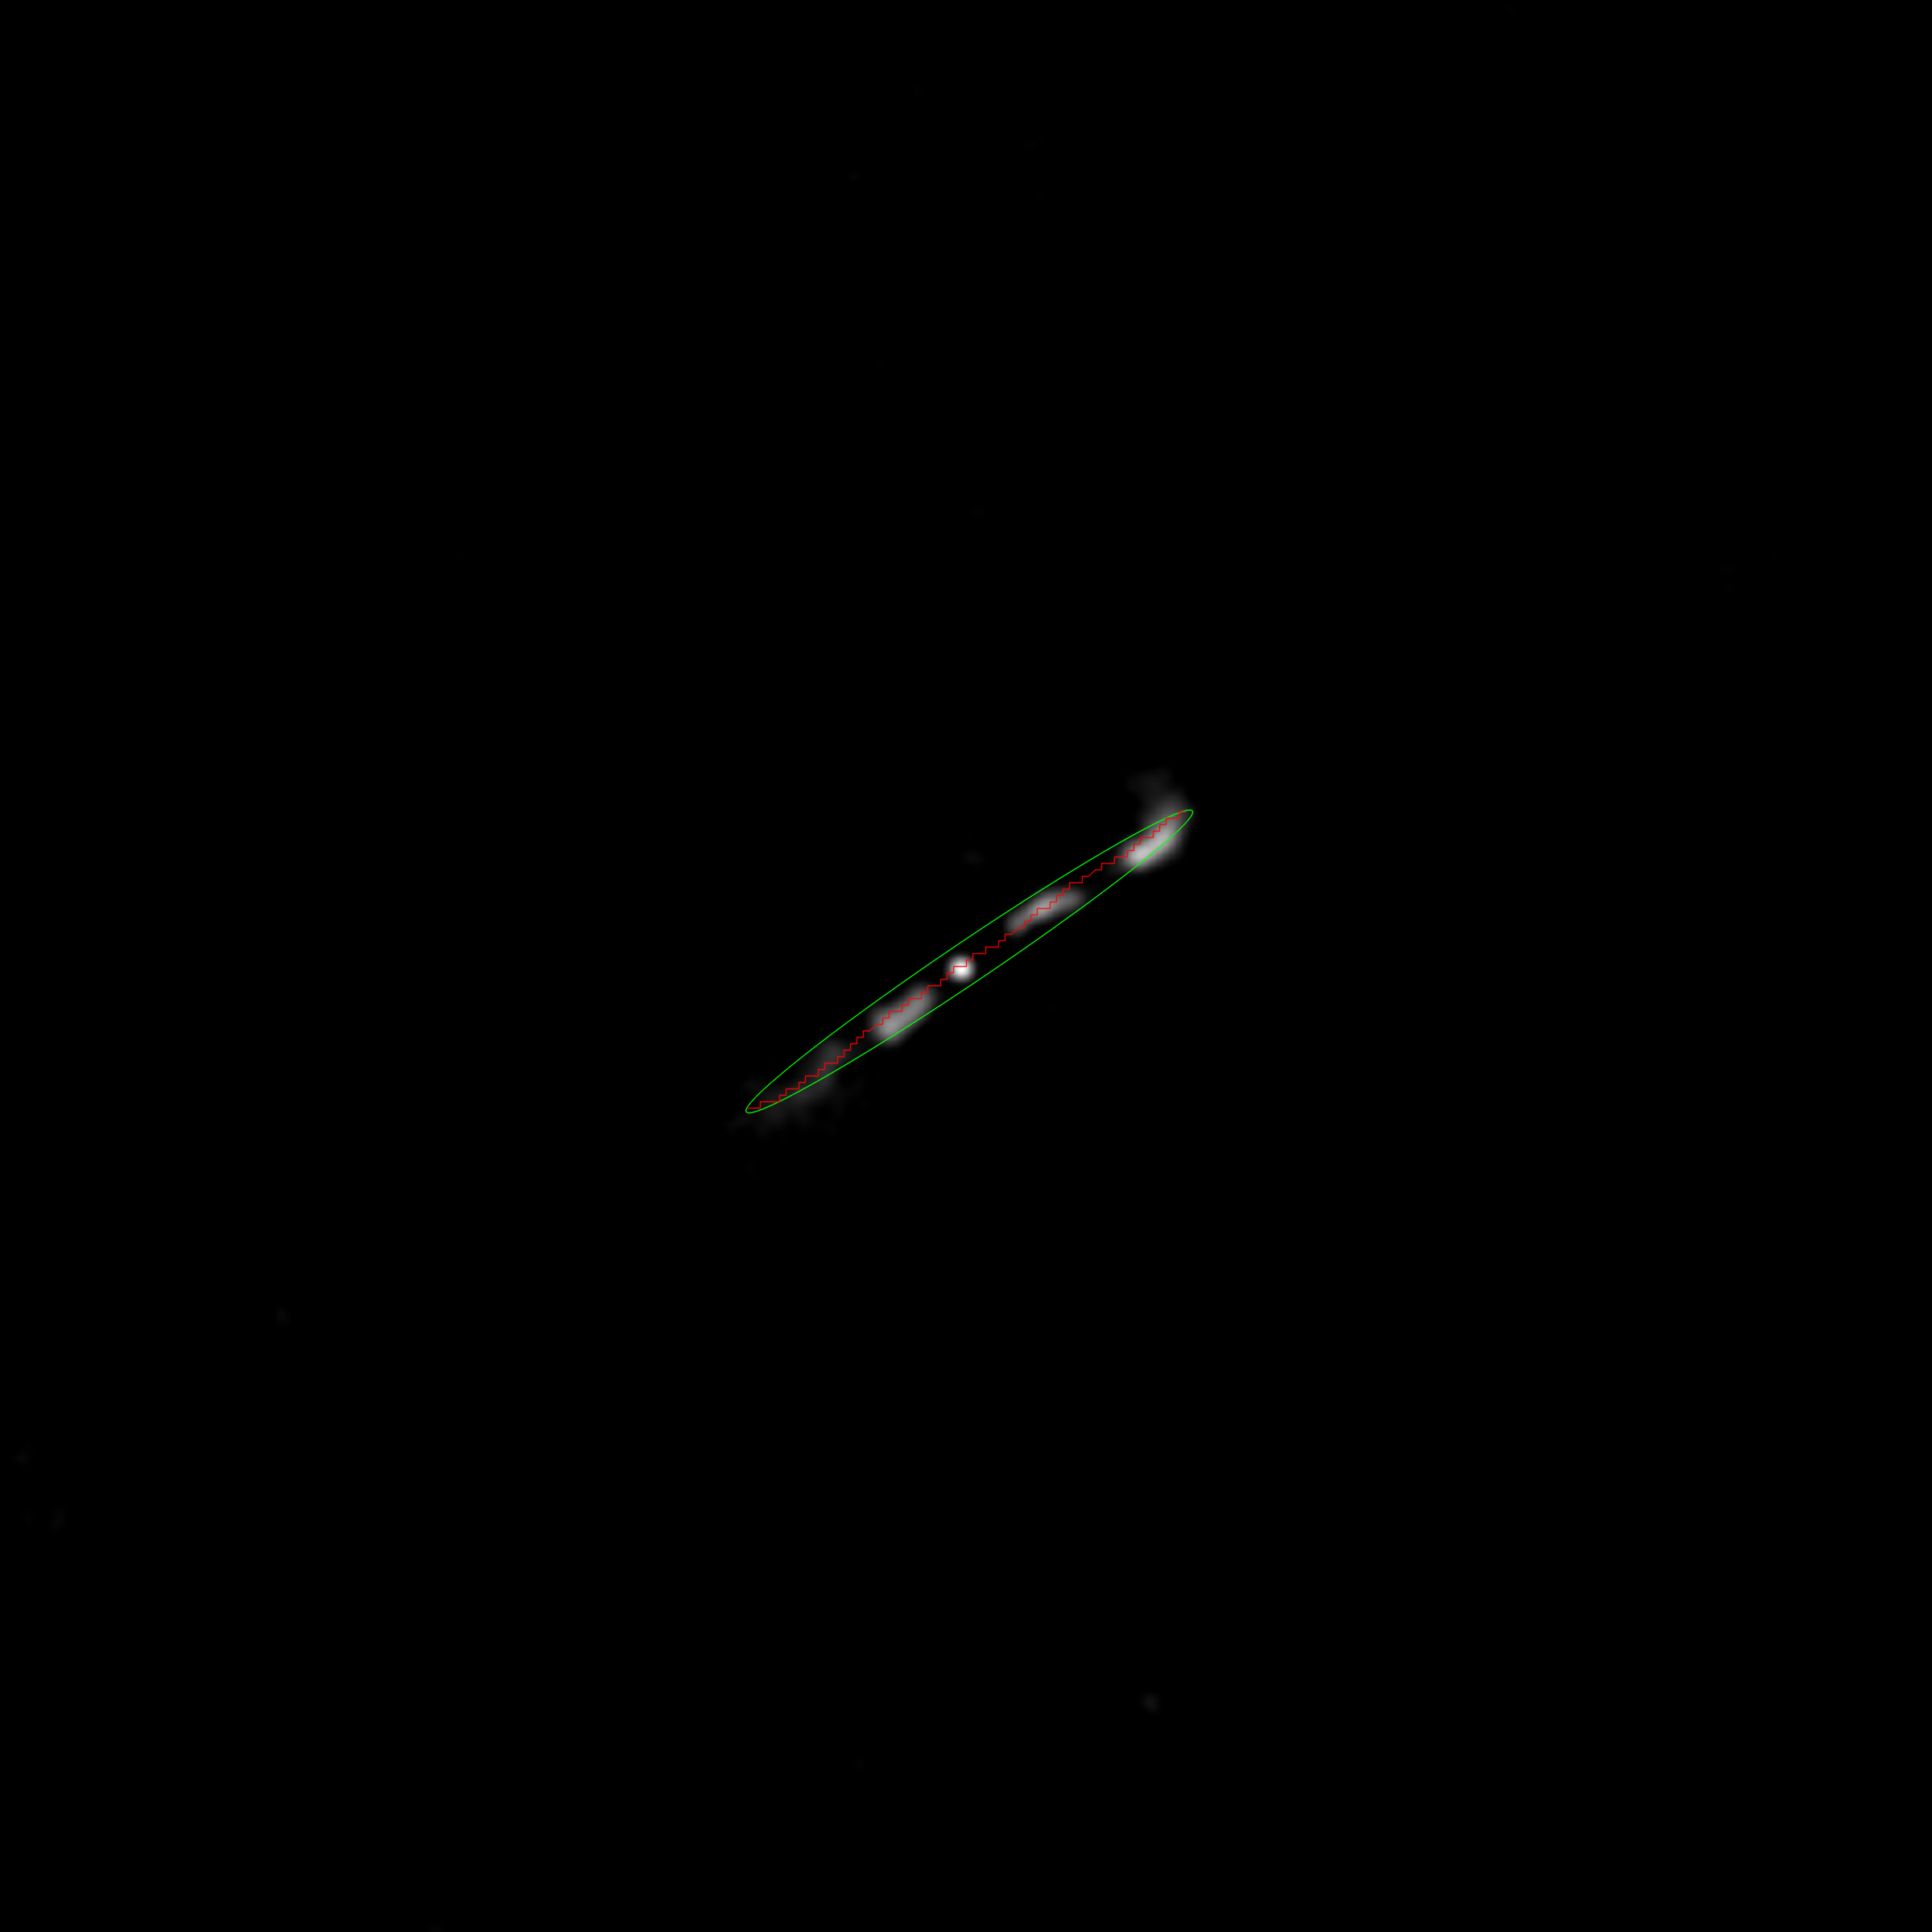
\includegraphics[clip, trim=800 800 800 800, scale=1.5, width=0.3\linewidth]{Figure/Section 3/149.318_19.114_0_MiraBest.png}
    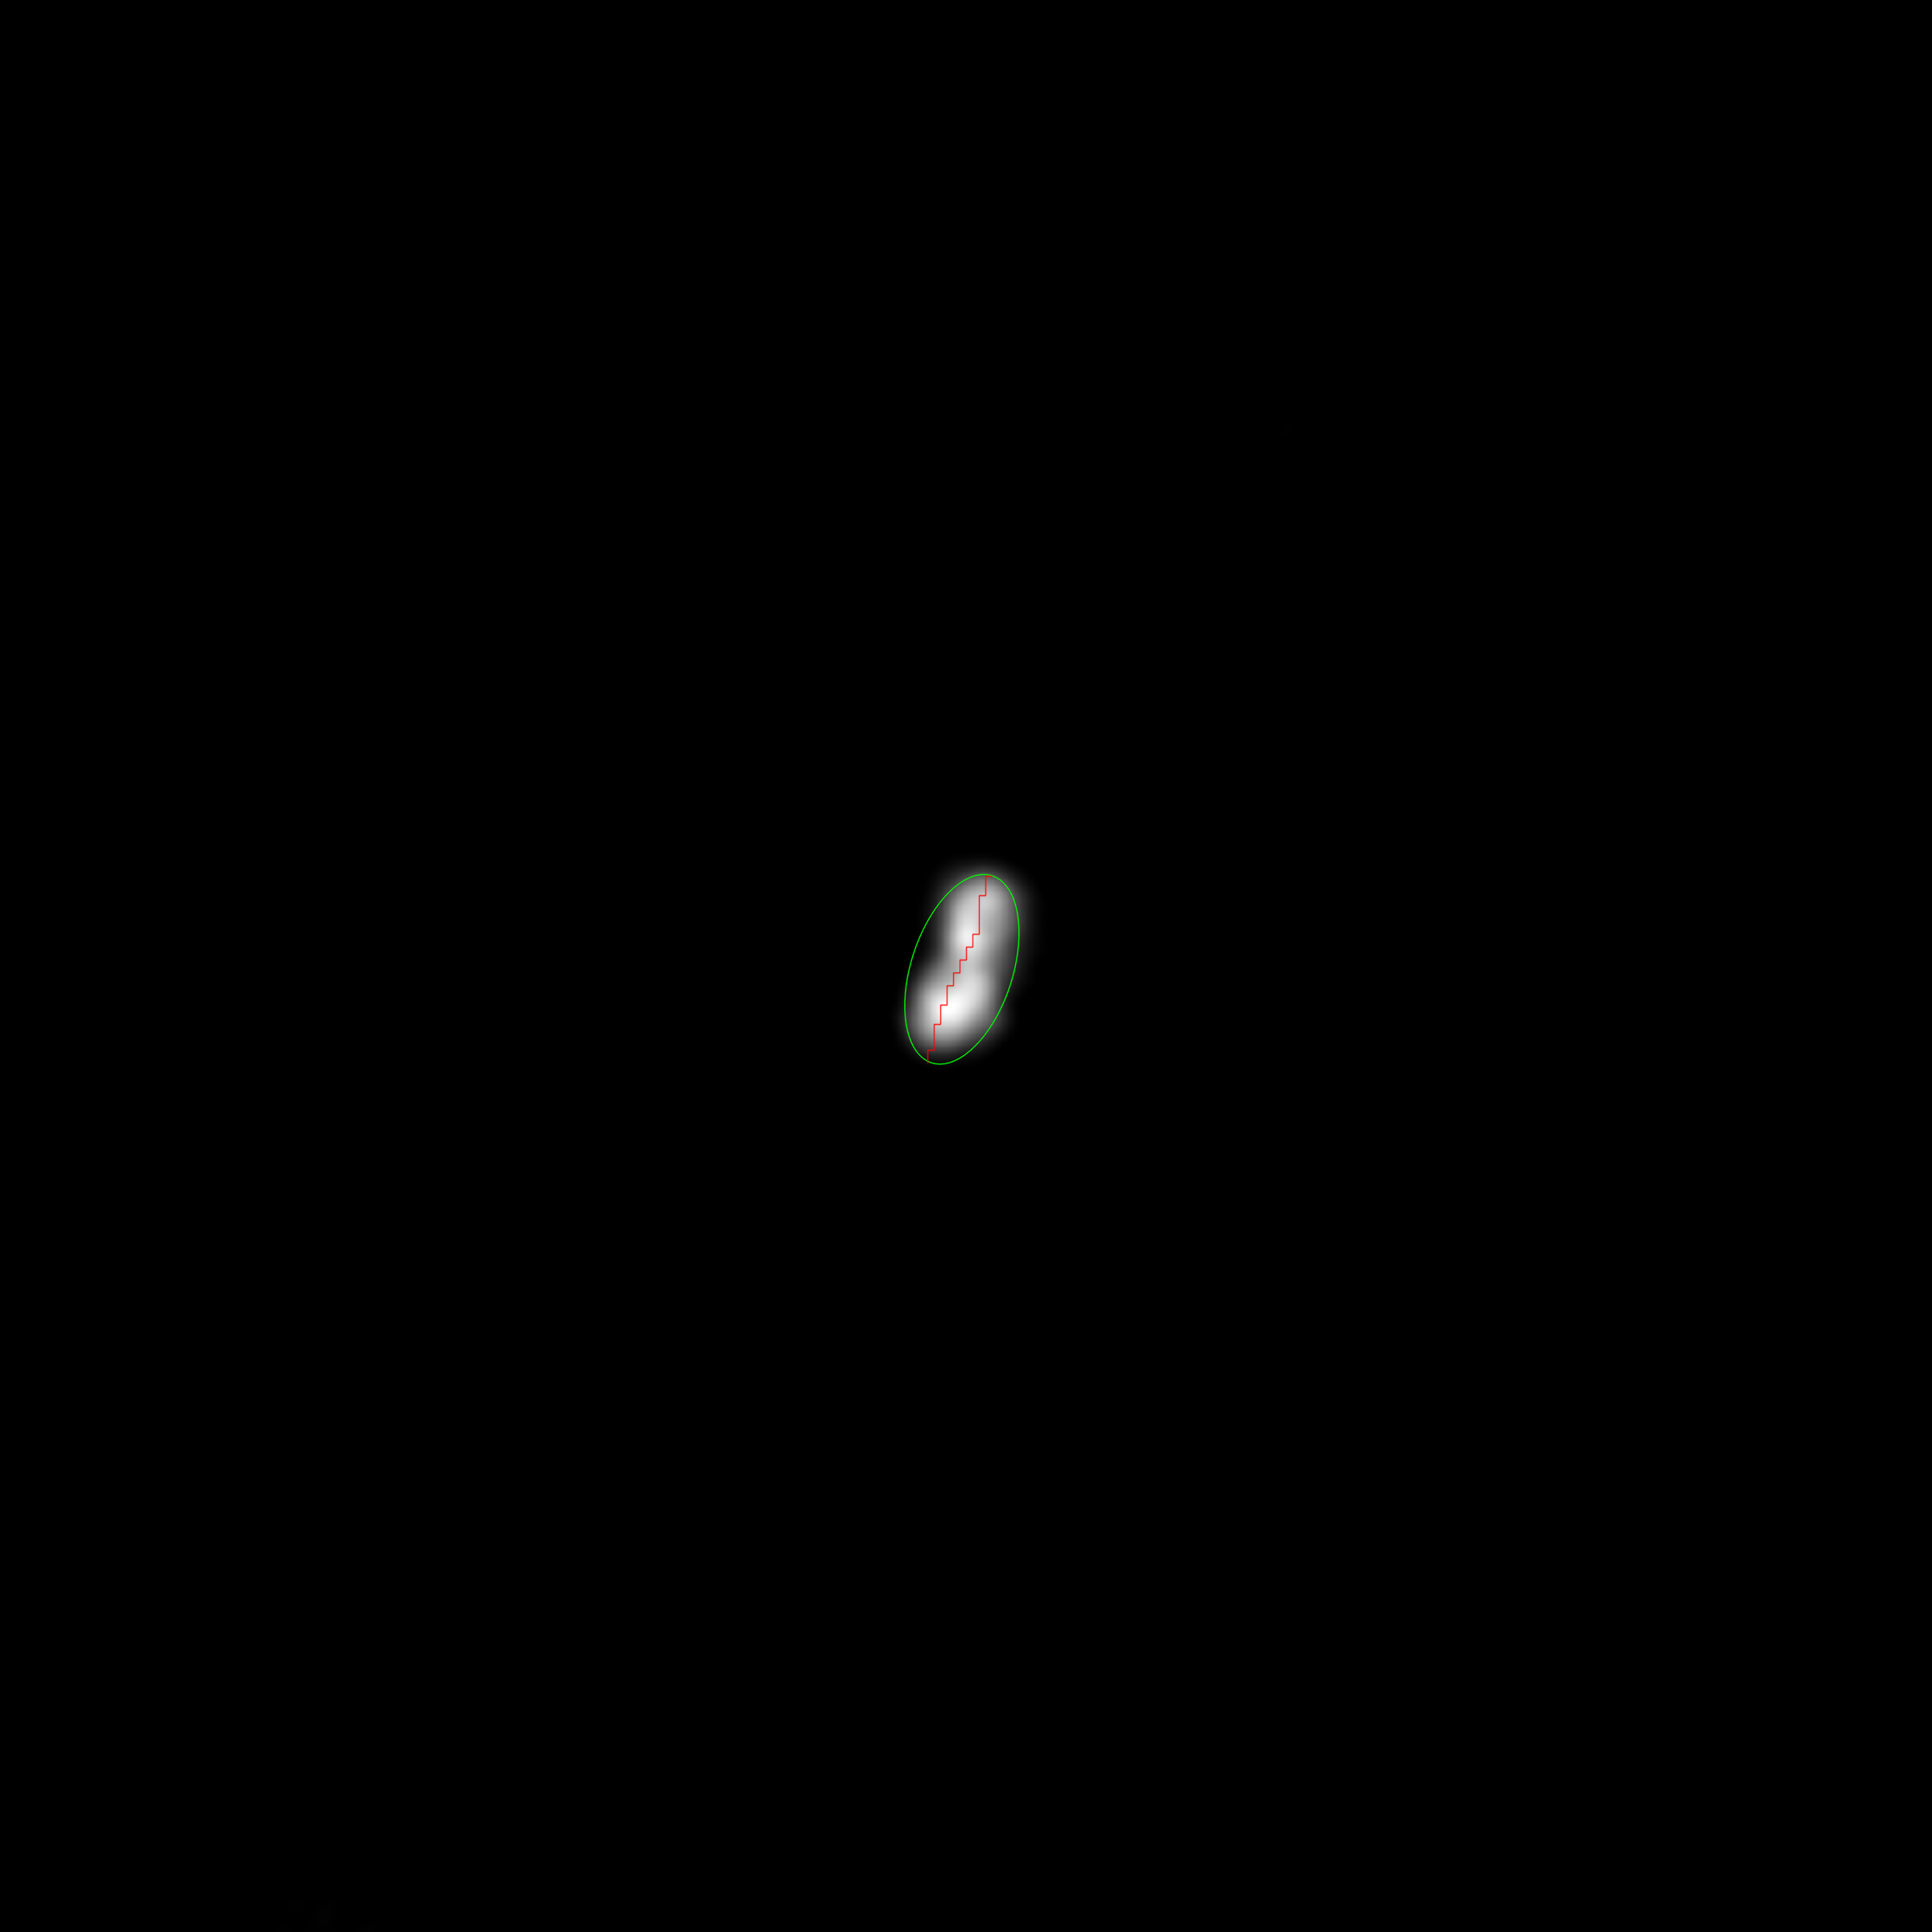
\includegraphics[clip, trim=1000 1000 1000 1000, scale=1.5, width=0.3\linewidth]{Figure/Section 3/150.738_19.865_0_Gendre.png}
    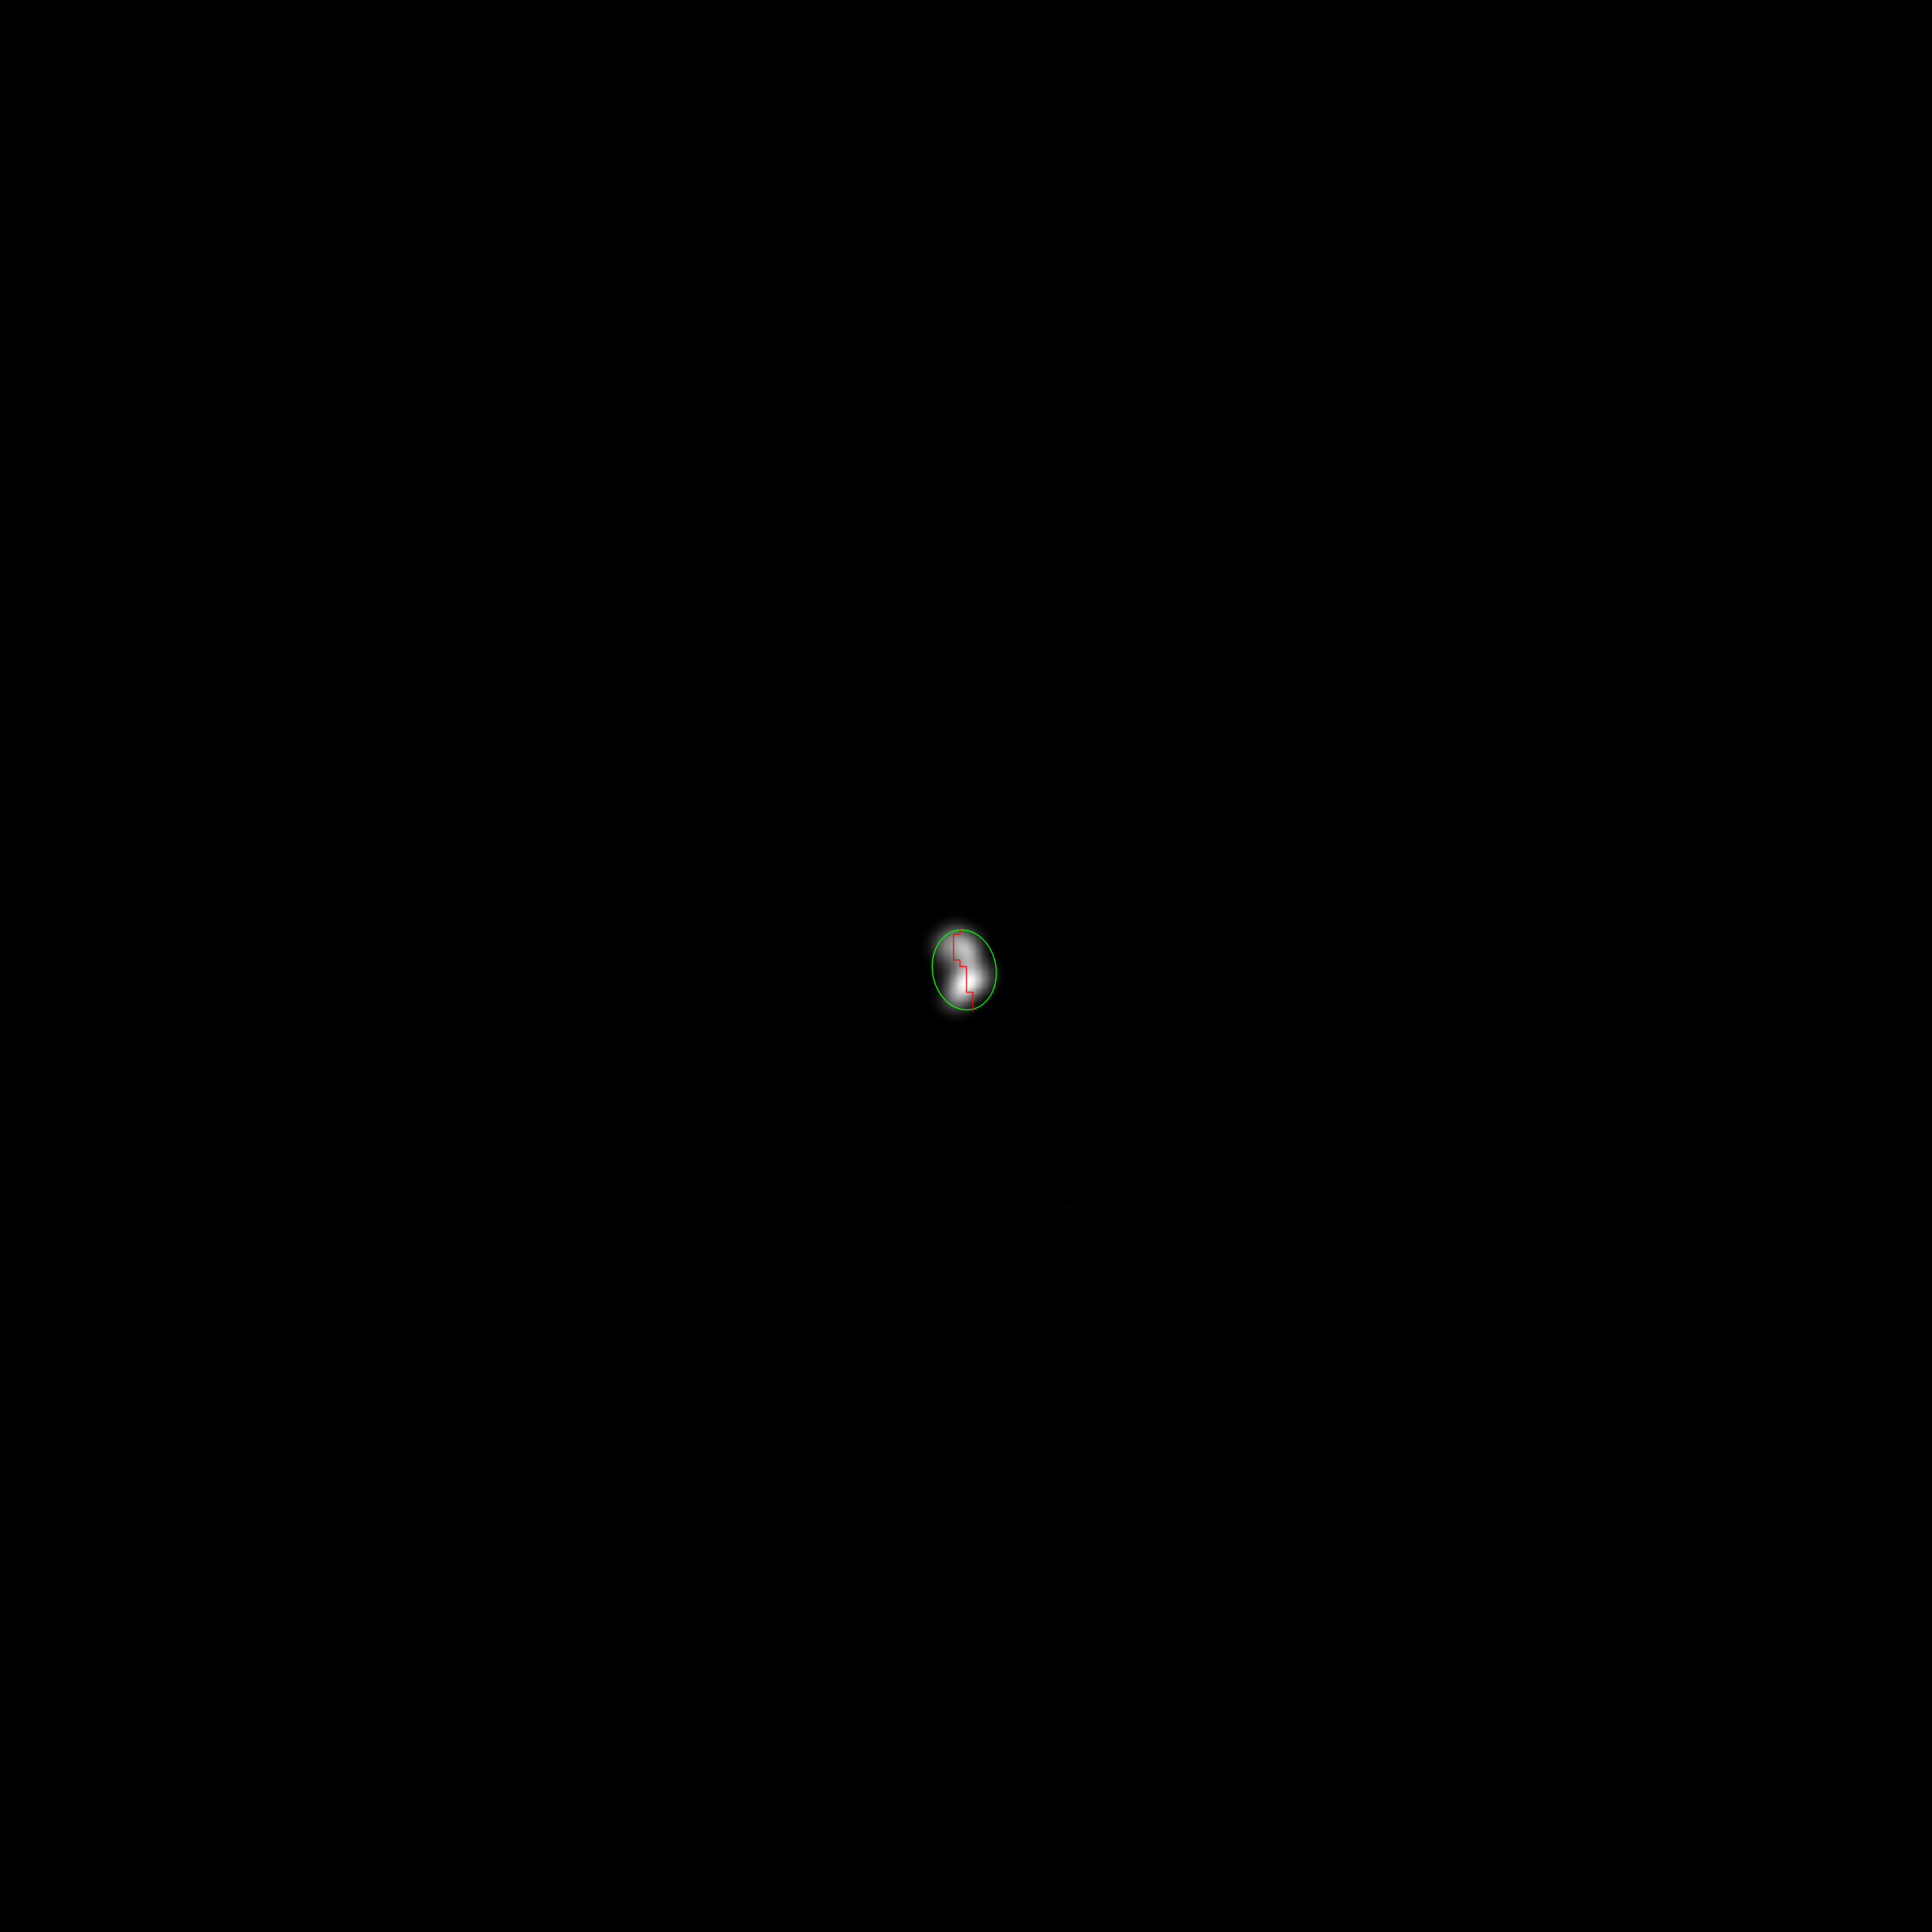
\includegraphics[clip, trim=1080 1080 1080 1080, scale=1.5, width=0.3\linewidth]{Figure/Section 3/228.764_22.529_0_Gendre.png}
    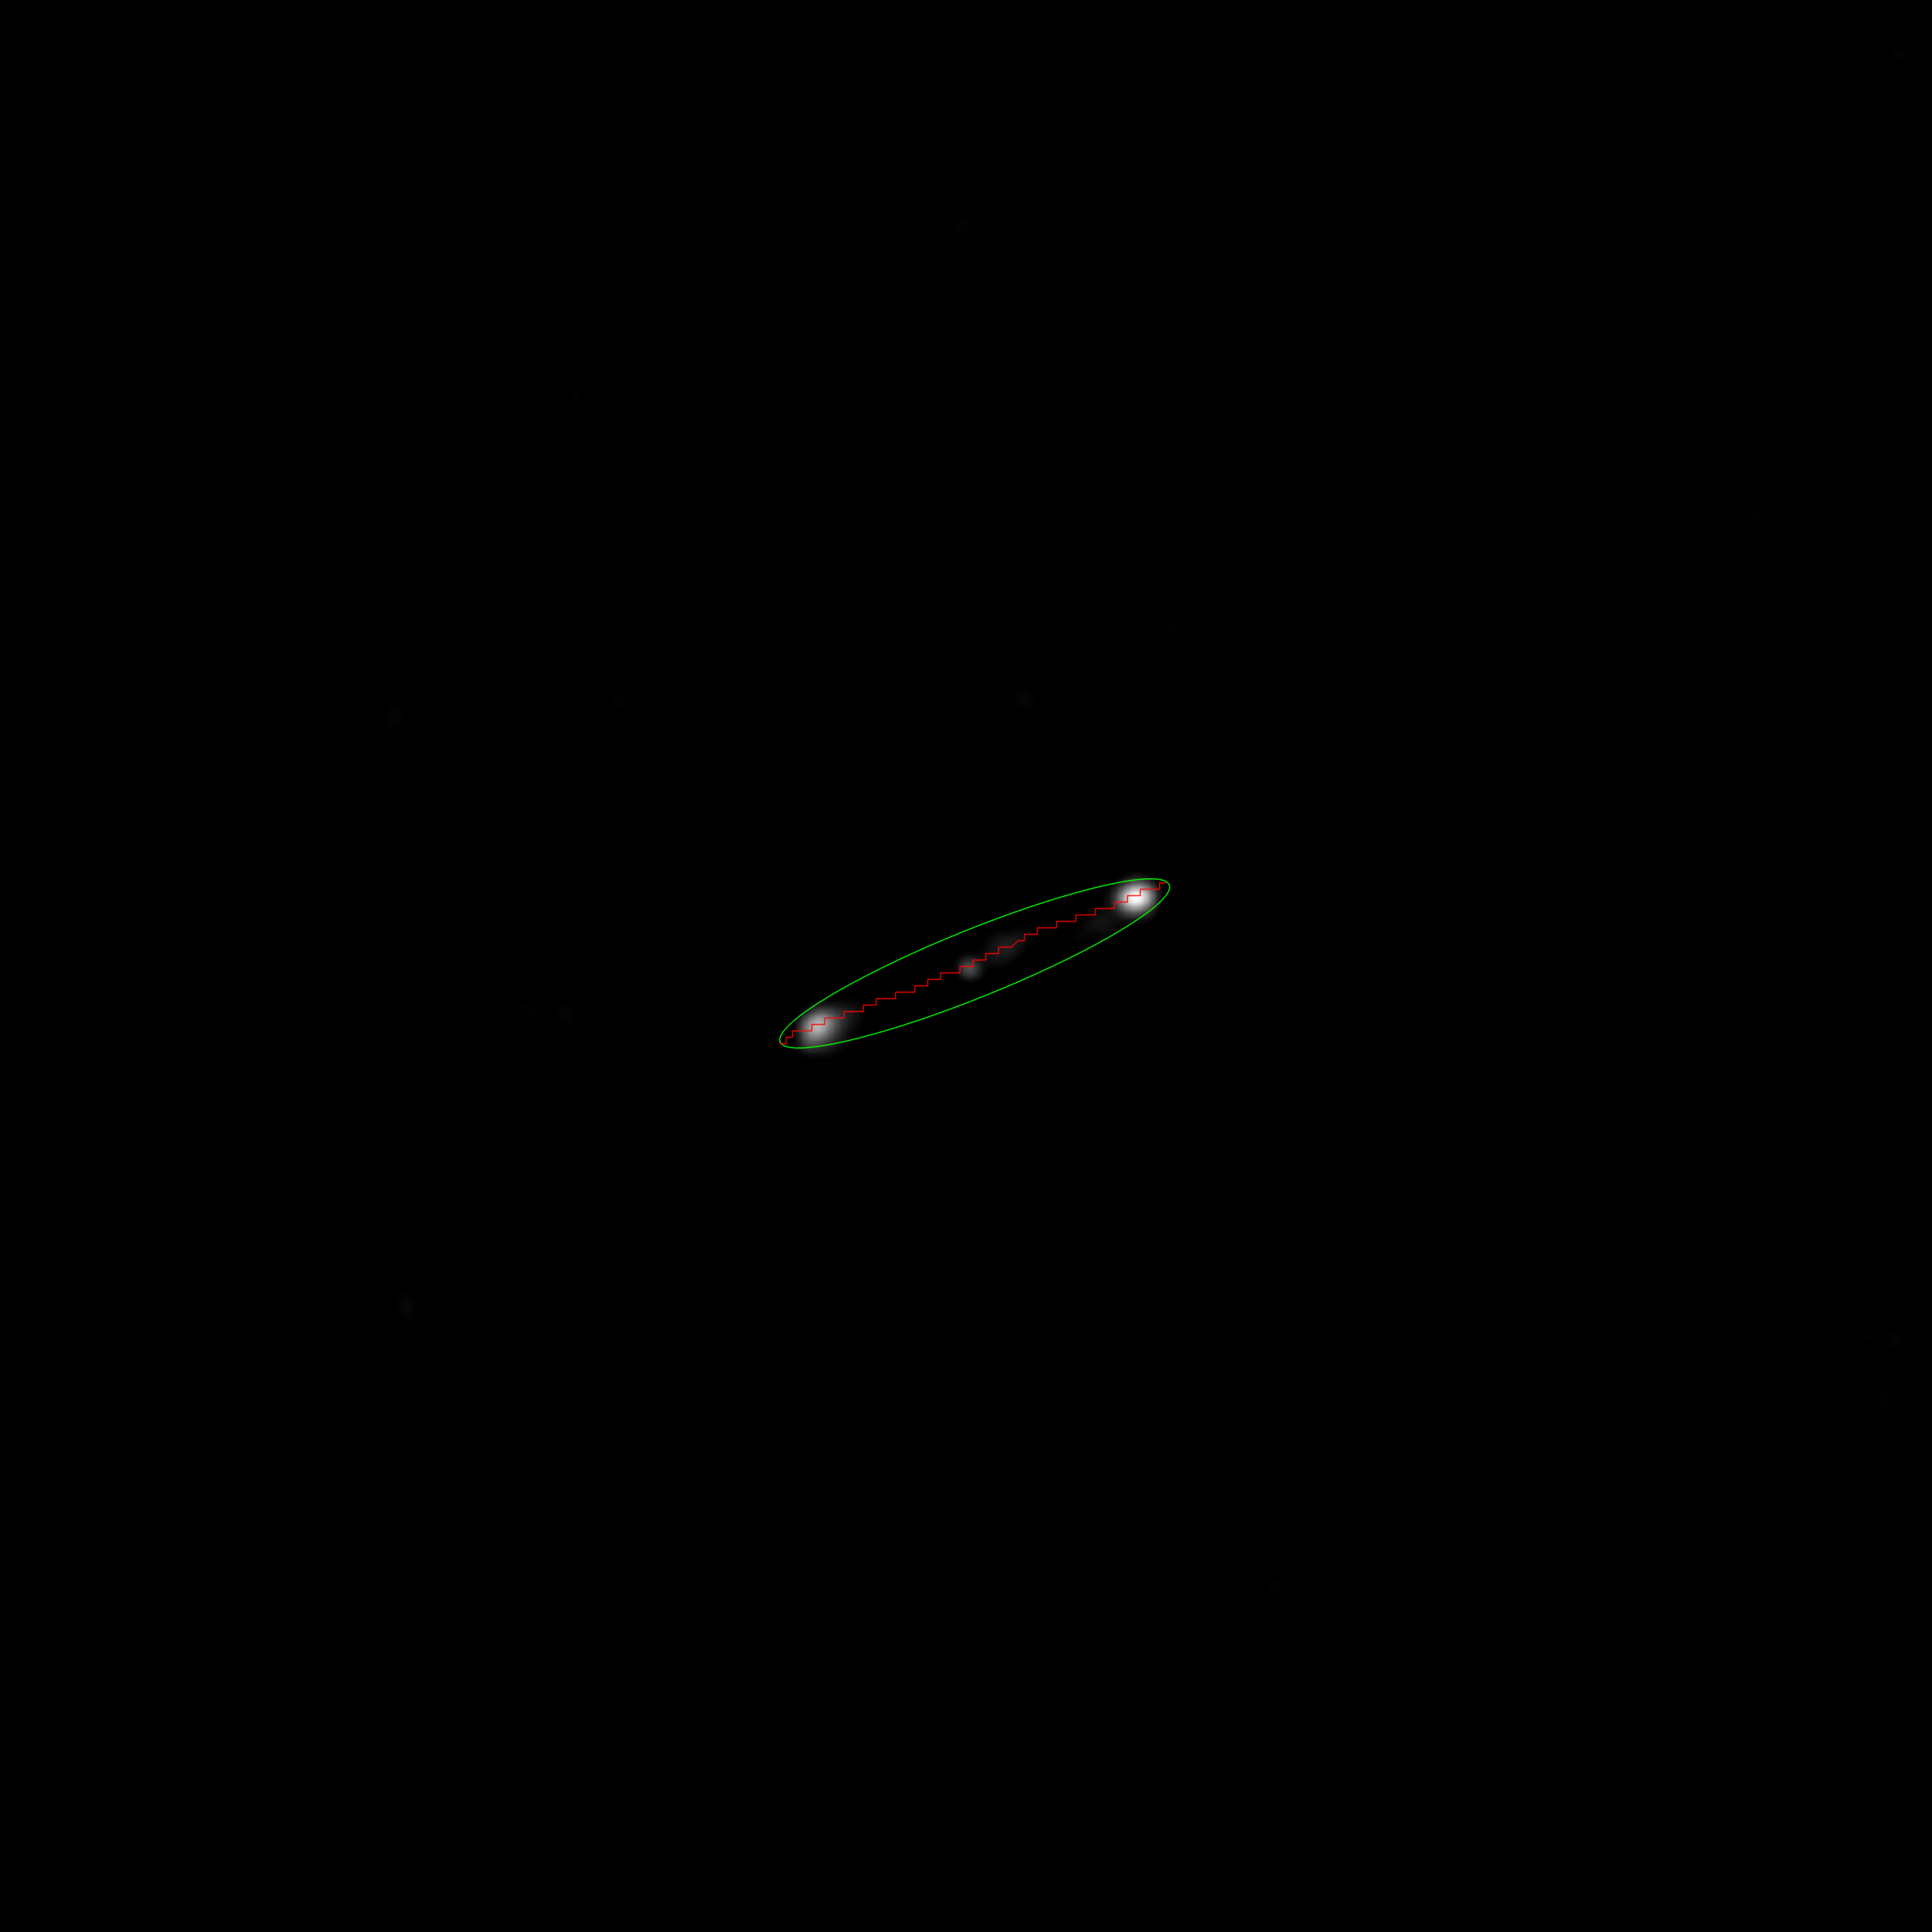
\includegraphics[clip, trim=920 920 920 920, scale=1.5, width=0.3\linewidth]{Figure/Section 3/180.424_22.946_1_MiraBest.png}
    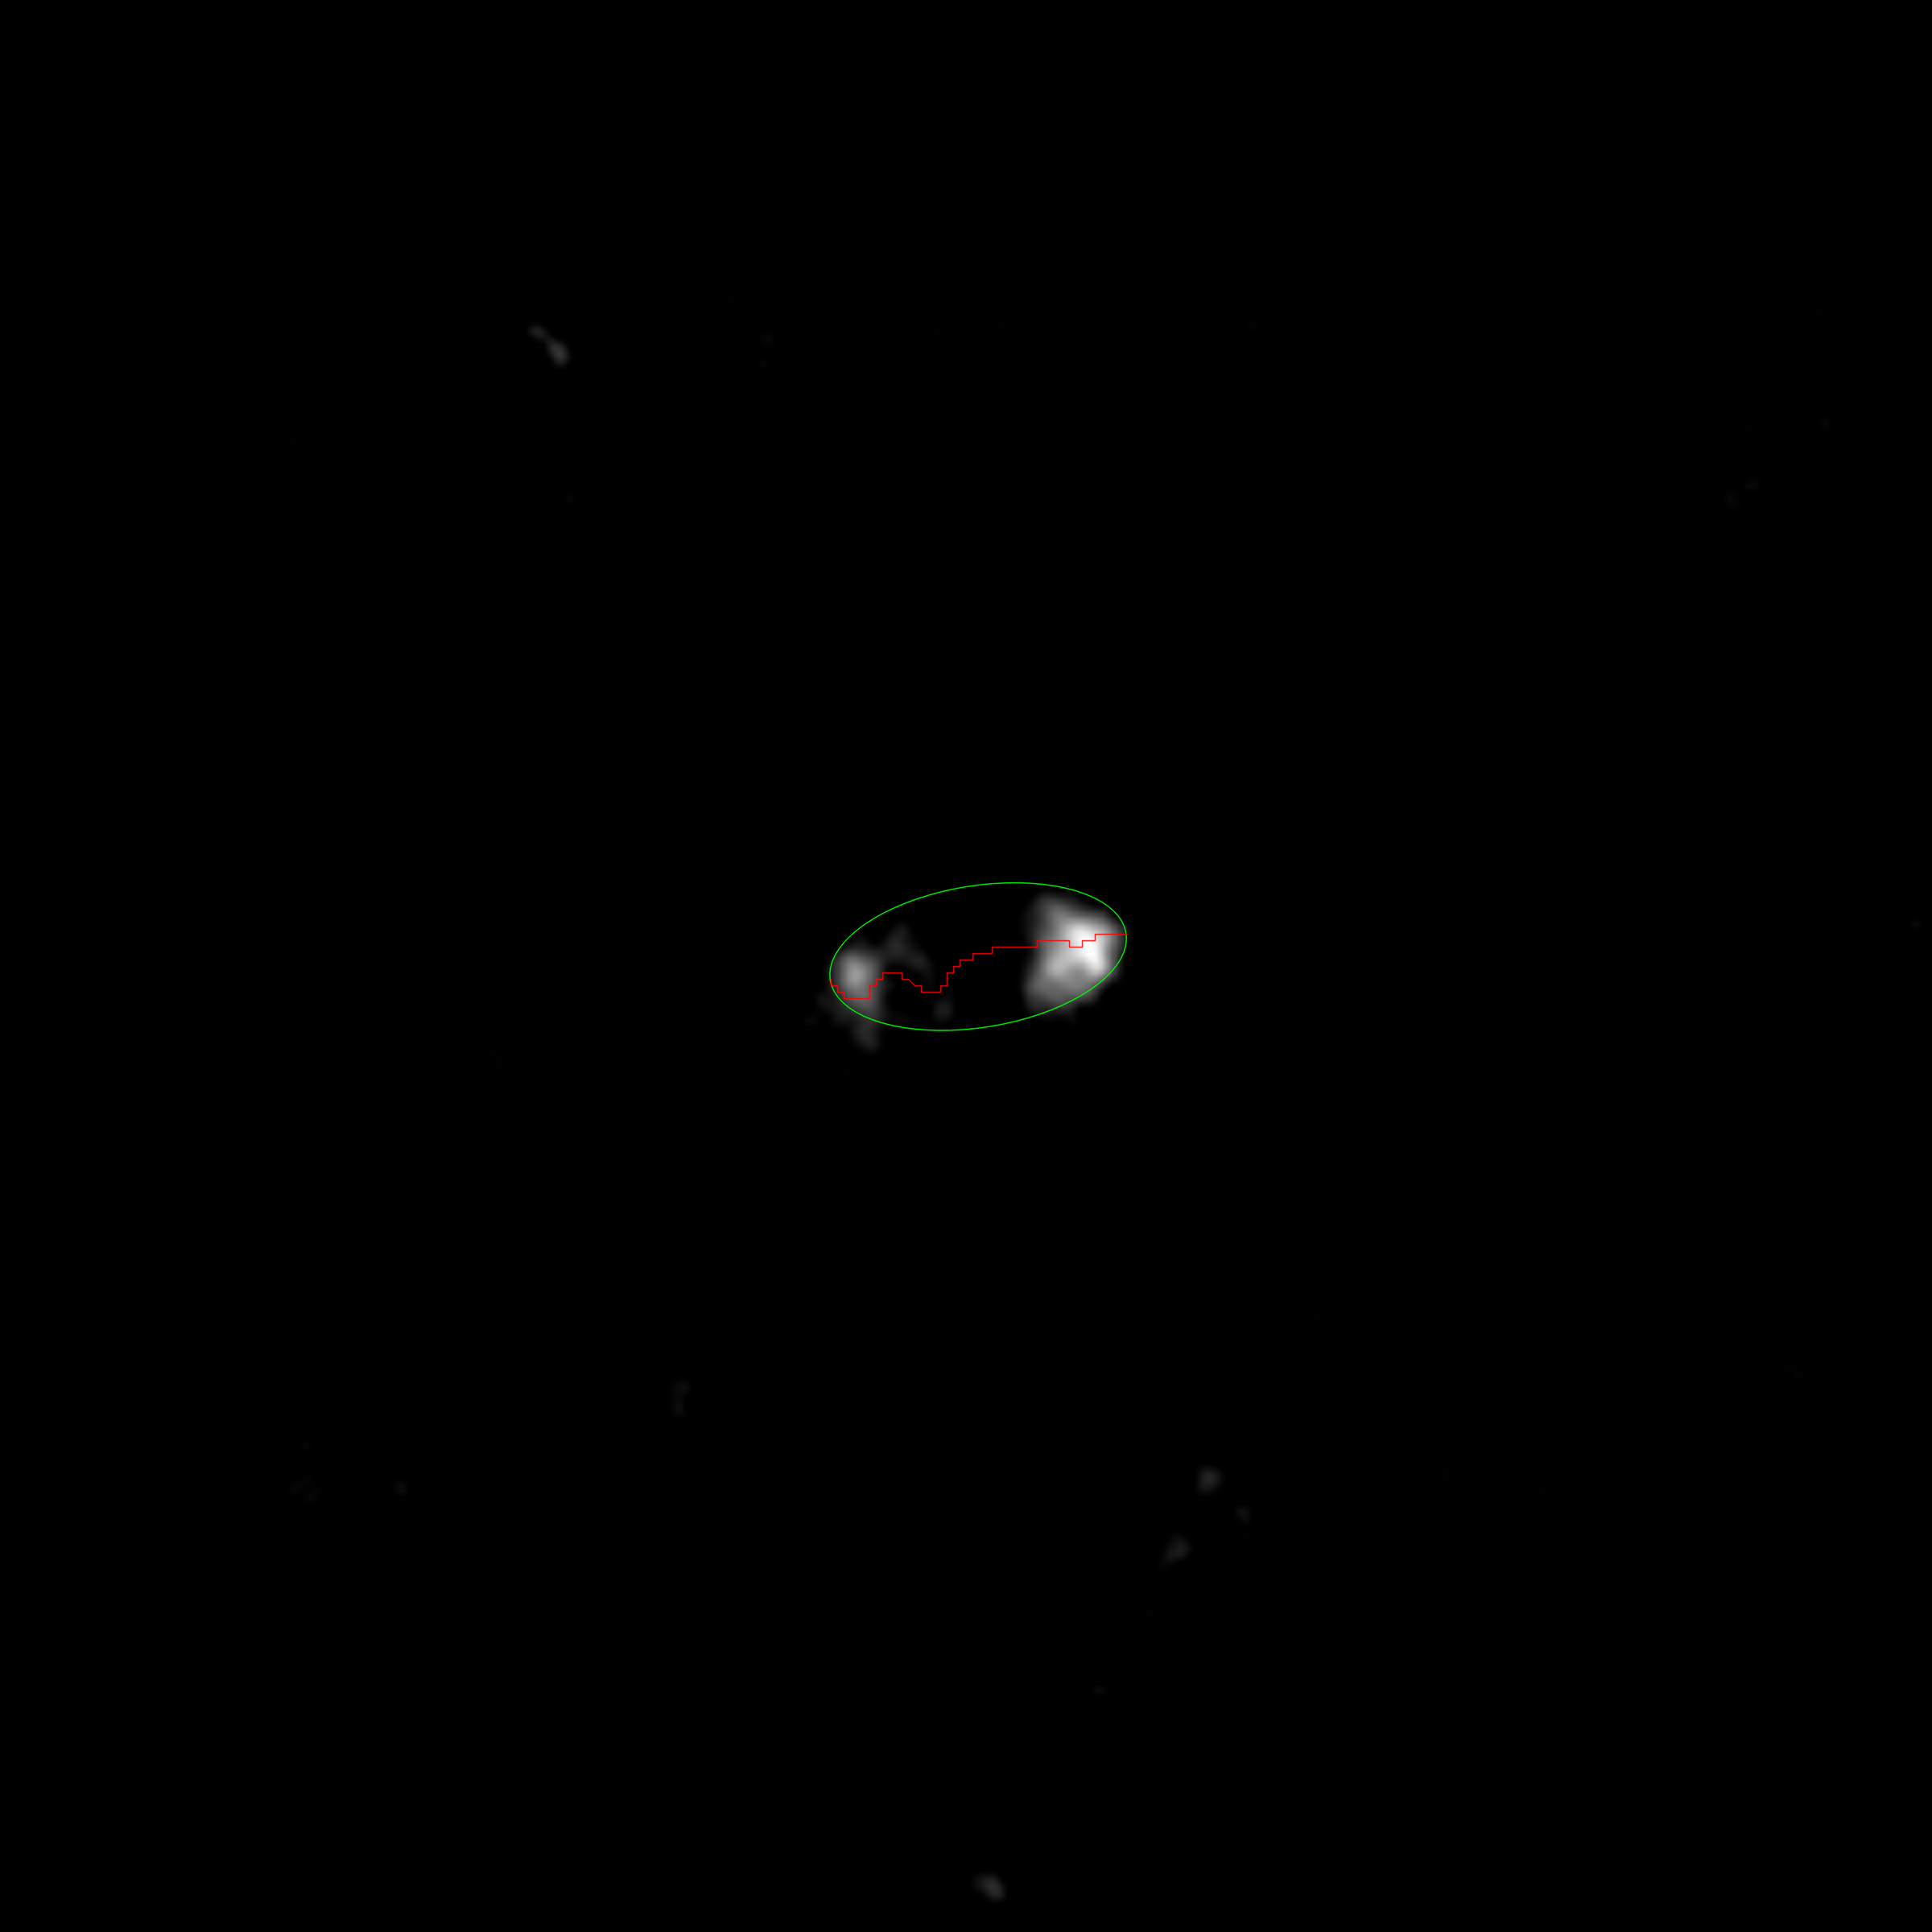
\includegraphics[clip, trim=960 960 960 960, scale=1.5, width=0.3\linewidth]{Figure/Section 3/213.728_22.633_1_MiraBest.png}
    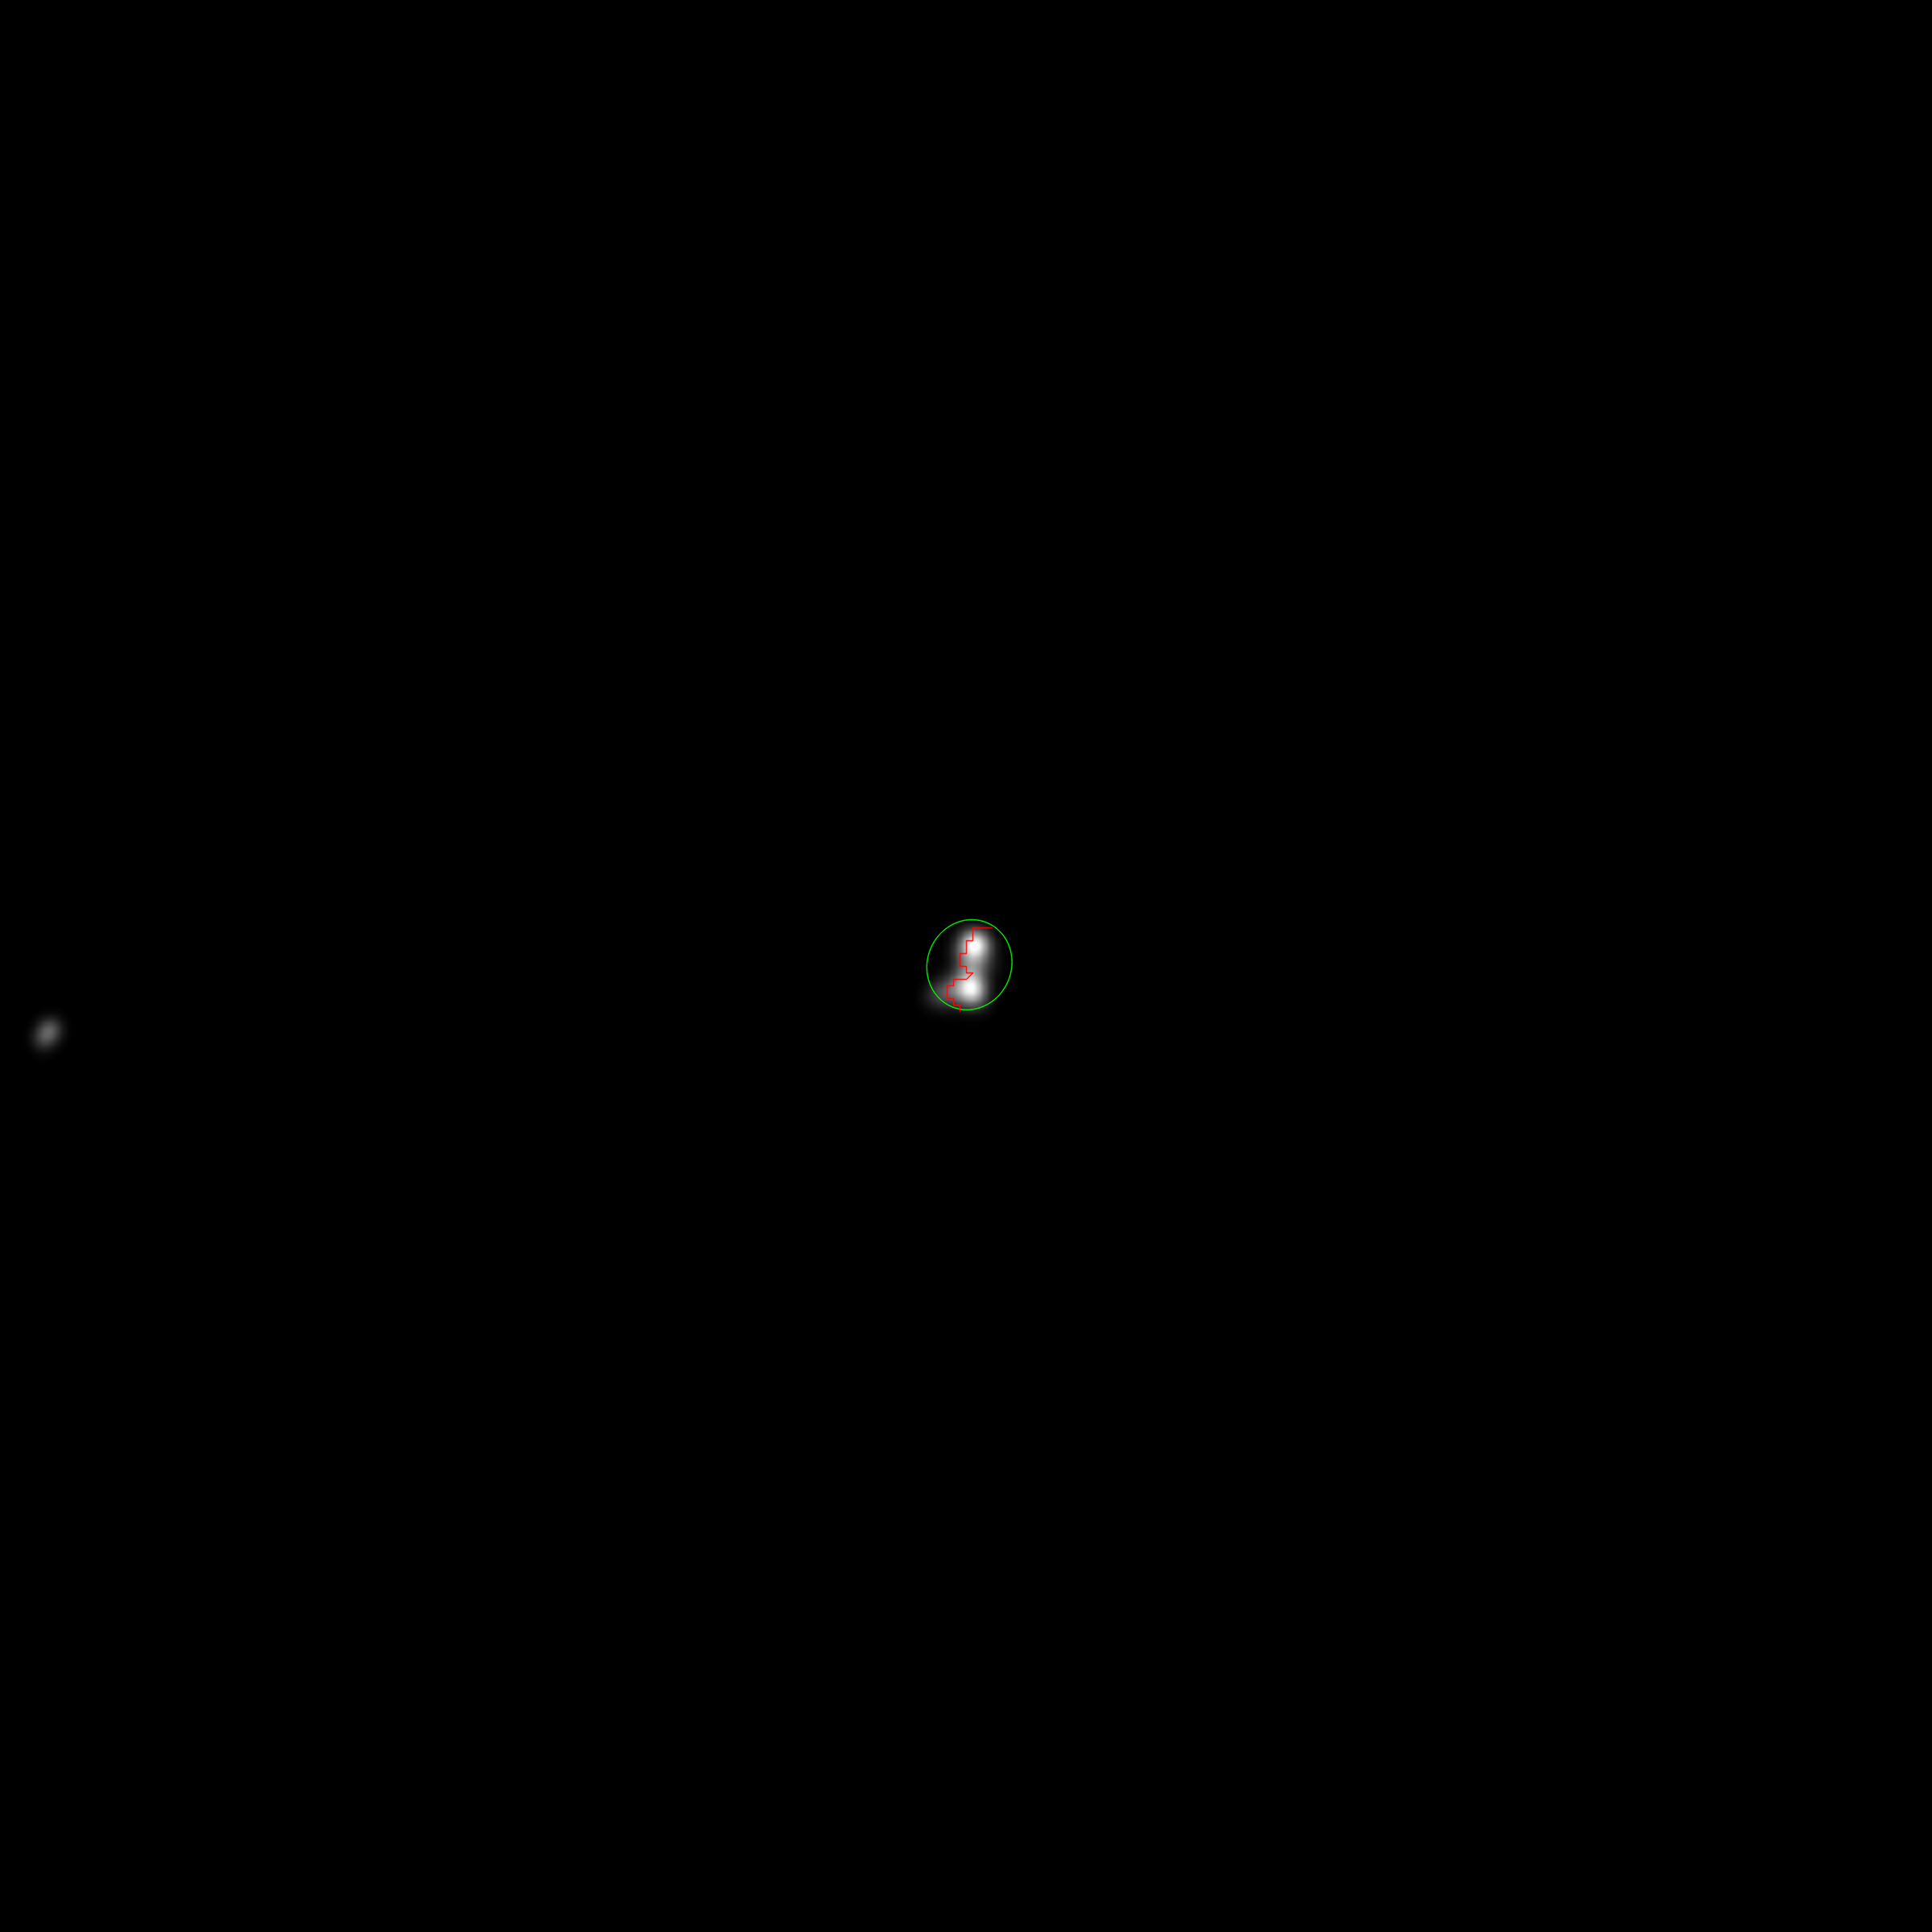
\includegraphics[clip, trim=1080 1080 1080 1080, scale=1.5, width=0.3\linewidth]{Figure/Section 3/125.391_47.043_1_Gendre.png}
    \caption{
    Top Panel: showing the FRI.
    Bottom Panel: showing the FRII.
    The green ellipse represents the algorithm-identified RG ellipse, while the red curve corresponds to the central line of the RG.
    }
    \label{fig:Figure2}
\end{figure}

%To position the core of RGs, an effective approach leverages optical host galaxy positional data. For example, when searching for target galaxy-associated sources, \citep{kumar_growth_2022} used NED’s gravitational wave follow-up service to conduct quick-look searches for candidates. Similarly, NED is used here to find optical counterparts and retrieve their data. In \autoref{sec:Section3_1}, the sample’s filtered optical counterparts show redshift distributions (see \autoref{fig:Redshift&MassDistribution}), with most redshifts < z=1. Optical counterpart mass and redshift data originate from catalogs archived in VizieR. This becomes challenging when multiple catalogs correspond to one optical counterpart, one catalog includes multiple estimation methods, or both; thus, the average mass is used for individual RGs. Naturally, data with both central black hole and stellar mass measurements is more representative\textemdash entries lacking either were excluded. In \autoref{fig:Redshift&MassDistribution}, the central black hole mass and galaxy stellar mass data for FRIs and FRIIs in the sample exhibit a slight degree of misalignment. However, their distribution ranges are so similar that this stands in sharp contrast to the subsequently analyzed parameters with significant differences.


\begin{figure*}[!htbp]
    \centering
    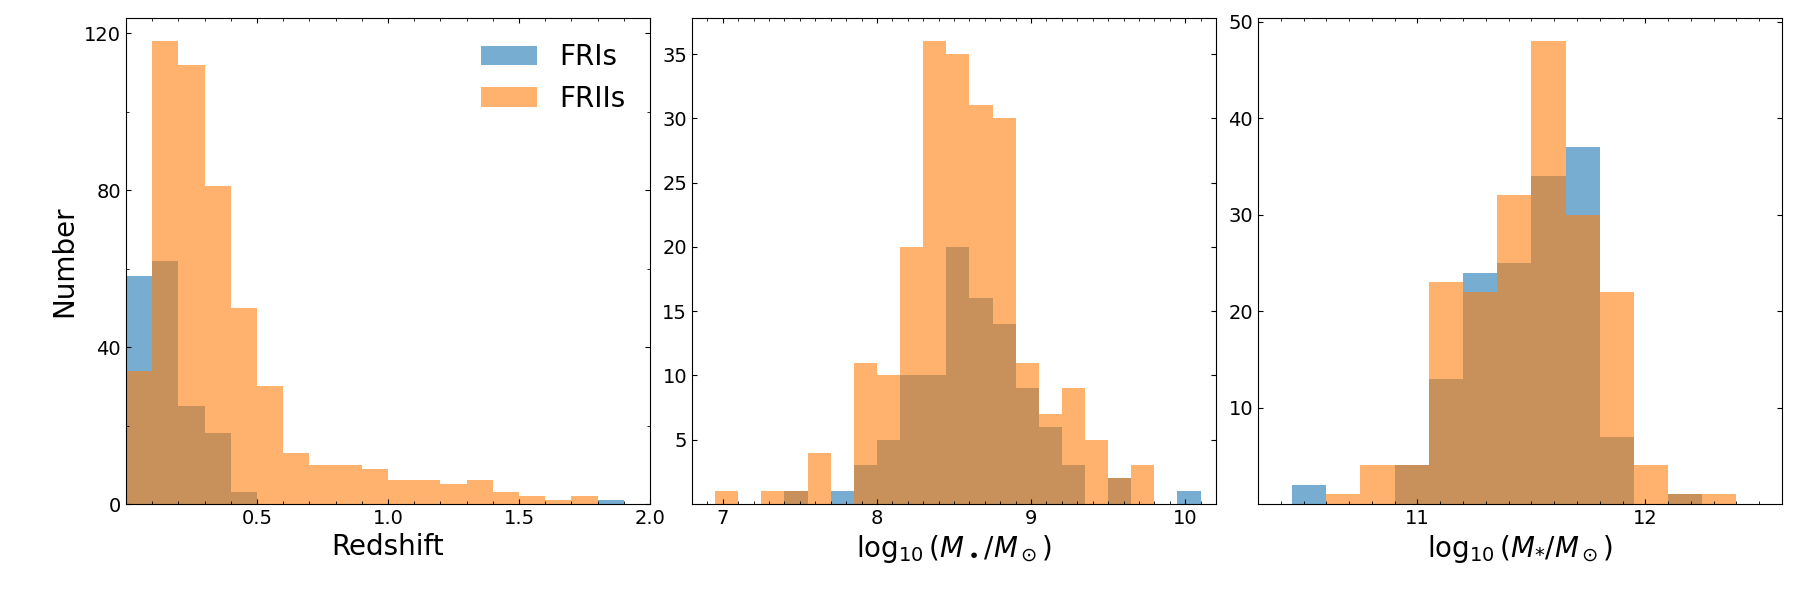
\includegraphics[width=0.9\linewidth]{Figure/Section 3/Redshift&MassDistribution.png}
    \caption{Here, we present the distributions of RGs with identifiable optical counterparts selected from our visually screened sample. The blue and orange histograms represent FRIs and FRIIs, respectively, and this color convention is used consistently throughout all subsequent figures. \textbf{Left}: Redshift distribution, comprising 169 FRIs and 506 FRIIs. \textbf{Middle}: Distribution of central black-hole masses for the subsample with available estimates, comprising 101 FRIs and 217 FRIIs. \textbf{Right}: Distribution of host-galaxy stellar masses for the subsample with available estimates, comprising 147 FRIs and 192 FRIIs. All mass estimates are mean values calculated from the measurements available for the corresponding optical counterparts in VizieR.}
    \label{fig:Redshift&MassDistribution}
\end{figure*}



%\subsection{Flood-filling Algorithm}\label{sec:Section3_3}
%To extract the contours of RGs, employing the Flood-filling algorithm serves as an effective method for determining the extent of the associated RG \citep[e.g.,][]{mingo_revisiting_2019,hales_blobcat_2012}; Starting from known internal points, the Flood-filling algorithm only expands to adjacent non-boundary points, while boundary points are consistently excluded; this facilitates the identification of the contours of RGs under specific conditions \citep{lieberman_how_1978,fishkin_family_1984}. In this procedure, it is specified that the Flood-filling algorithm will disperse seed points in all connected regions of the image with non-zero brightness, while the brightness threshold is set to 5\% of the brightness value of the brightest point in the image.


%\subsection{Principal Component Analysis}\label{sec:Section3_4}
%Most applications of PCA in astronomy relate to identifying eigenvectors across a population of objects \citep[e.g., PCA tomography][]{steiner_pca_2009}, PCA will be employed to detect the principal direction that best align with RG structures in the context of the present work. PCA is a powerful technique for extracting structure from potentially high-dimensional datasets, and a small number of principal components is often sufficient to account for most of the structural information in the data \citep{hofmann_kernel_2008}. Specifically, for the morphological analysis of RGs\textemdash whose observational data typically encompasses multidimensional information (e.g., spatial coordinates and brightness gradients)\textemdash PCA integrates these discrete data points into a low-dimensional principal component space. It prioritizes and preserves the information driven by the highest variance while filtering out noise and redundant signals unrelated to morphology. In this paper, in addition to the targeted RGs, other radio sources (e.g., compact sources) present in the acquired FIRST images interfere with the processing of the target. Compared with RGs, these interfering sources exhibit simpler structures and significantly smaller scales. Consequently, when PCA is employed to process the brightness distribution, the variance corresponding to the identified largest distribution direction is substantially greater than that of the second largest variance. PCA enables the direct retrieval of the core morphological features of RGs without relying on complex auxiliary data, which aligns with the previously outlined requirement for efficient and concise morphological extraction.


%The Central Line derived via skeletonization is proposed as a structural reference for RG systems. PCA aids in identifying representative clumps; however, these clumps cannot be readily interpreted as the full RG system, and their structural validity requires further verification. The processed central-line structure is illustrated in \autoref{fig:Redshift&MassDistribution}. After excluding significant deviations, the most complete RG system structures and their associated optical counterpart information are retained.

%Skeletonization is a well-established method for image structure characterization, and Breadth-First Search (BFS) enables the identification of the central line of RG skeleton\textemdash this line, in turn, facilitates the simplification of the features of the RG's brightness distribution. Skeletonization enables efficient compression of RG structure while preserving its core structural information. Specifically, using iterative skeletonization methods, foreground regions can be reduced to single-pixel-wide skeletons while maintaining topological features; for analogous work, see \cite{vardoulaki_fr-type_2021}. Then, BFS algorithm enables the identification of a line within the skeletonization process that characterizes the center of RG brightness distribution. This constitutes a pruning process, as extraneous branches in the skeleton are irrelevant for characterizing the overall orientation of lobe structures. Thus, BSF algorithm can retain the primary backbone\textemdash most representative of lobe structure\textemdash hereafter referred to as the central line. Merely applying BFS algorithm alone is insufficient; it is additionally required to incorporate into the algorithm the constraint that the direction of the central line is roughly aligned with the PCA-derived principal direction, as well as the requirement that the central line passes through hot spots or other compact clumps.

%Notably, \cite{barkus_application_2021} employed analogous methodologies; however, their ridge lines \textemdash developed primarily for the identification and morphological classification of extended radio galaxies in radio astronomy  \textemdash may be less well-suited to RG systems featuring large structural gaps or curved head-tail configurations.


\begin{figure}[!htbp]
    \centering
    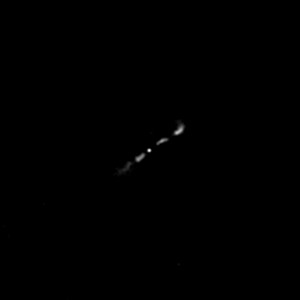
\includegraphics[clip, trim=100 100 100 100, scale=1.5, width=0.45\linewidth]{Figure/Section 3/origin_149.318_19.114_0_MiraBest.png}
    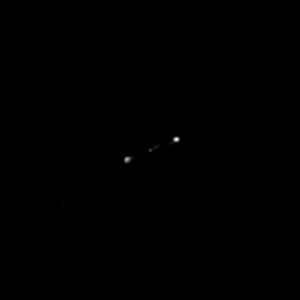
\includegraphics[clip, trim=100 100 100 100, scale=1.5, width=0.45\linewidth]{Figure/Section 3/origin_180.424_22.946_1_MiraBest.png}
    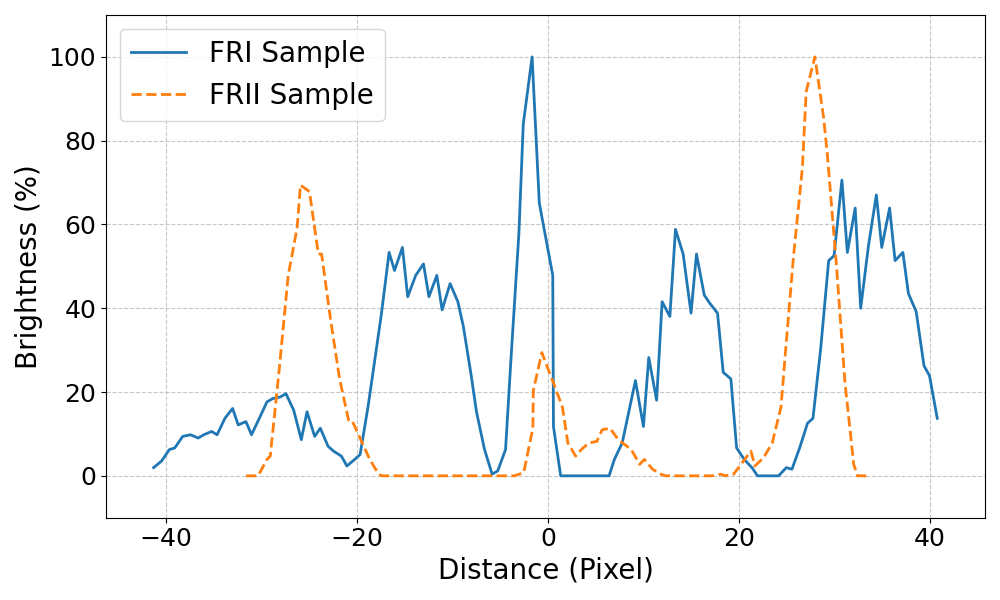
\includegraphics[width=1\linewidth]{Figure/Section 3/CenterLineLuminosity.png}
    \caption{Top left: FRI's sample (R.A. 149.318°, Dec. 19.114°);  Top right: FRII's sample (R.A. 180.424°, Dec. 22.946°);  Bottom: Luminosity distribution along the central line, with the peak brightness normalized to 100\%.}
    \label{fig:CentralLine}
\end{figure}



% 在这一方面的方法中，椭圆很重要，过去曾经有不少工作都用了椭圆结构
%Elliptical structures hold substantial significance in morphological studies of radio galaxies (RGs). A simple elliptical morphology has been repeatedly observed in prior analyses of RG structure \citep[e.g.,][]{lin_new_2024, carilli_cygnus_1996, begelman_overpressured_1989}. Evidently, elliptical structures serve as a general and effective descriptor for radio-loud sources.


%To enable independent modeling of the core region and lobes of RGs, \cite{lin_populations_2010} defined \(S\) as the angular separation between the peaks of highest surface brightness on either side of the host galaxy, designating \(T\) as the total linear size of the RG and thus defining \(r_s \equiv S/T\) as the primary metric for RG morphology. A key component of this approach involves fitting source components via Gaussian modeling; unfortunately, many sources in the dataset used in this study lack beam parameters consistent with those in the FIRST Catalog.
%To enhance the universality of the simulations, the methodology is simplified herein: 
%For FRIIs, hot spots are identified by locating the brightest points and outermost elliptical Gaussian components on opposite sides of the RG’s optical counterpart. Meanwhile, \(T\) is adopted as the maximum distance between the outermost pixels of the RG, a parameter that characterizes the overall size of the system. 
%For FRIs, \(S\) is defined as the major-axis size of the largest elliptical Gaussian component at the system’s center.


%Elliptical Gaussian models are fitted sequentially to decompose Gaussian components within the RG system. The process starts with an optimal single-component Gaussian fit; the modeled emission is subtracted from the original image, and fitting iterations continue on the residual image until at least 95\% of the brightness distribution is accounted for.
%Specifically, to optimally cover the entire RG, distinct strategies are adopted for different FR types. For FRI sources \textemdash featuring a bright core and the classic lobe–core–lobe morphology \textemdash a three-component elliptical Gaussian model is used to fit the central clump, decomposing it into one core and two lobes: the component with the highest brightness weight is designated as the core, and the other two as lobes. A minimum enclosing ellipse is then determined, tangent to the elliptical extents of the two lobes. For FRII sources, the RG ellipse is defined using elliptical Gaussian models of the hotspots: with the major-axis orientation fixed to the principal component direction, a minimum enclosing ellipse tangent to the hotspot elliptical boundaries is constructed.
%Ultimately, a minimum ellipse that optimally encloses the entire RG is identified for each FR type based on their distinct morphological structures.


%The process outlined above is illustrated in \autoref{fig:Different_rs}. Meanwhile, \autoref{fig:Figure2} specifically presents the elliptical structure derived from the processing workflow shown in \autoref{fig:FR_type_operate}. The equatorial coordinates (R.A. , Dec.) of these radio galaxies are as follows: (149.318°, 19.114°), (150.738°, 19.865°), (175.545°, 55.458°), (180.424°, 22.946°), (213.728°, 22.633°), (125.391°, 47.043°).


\begin{figure}[!htbp]
    \centering
    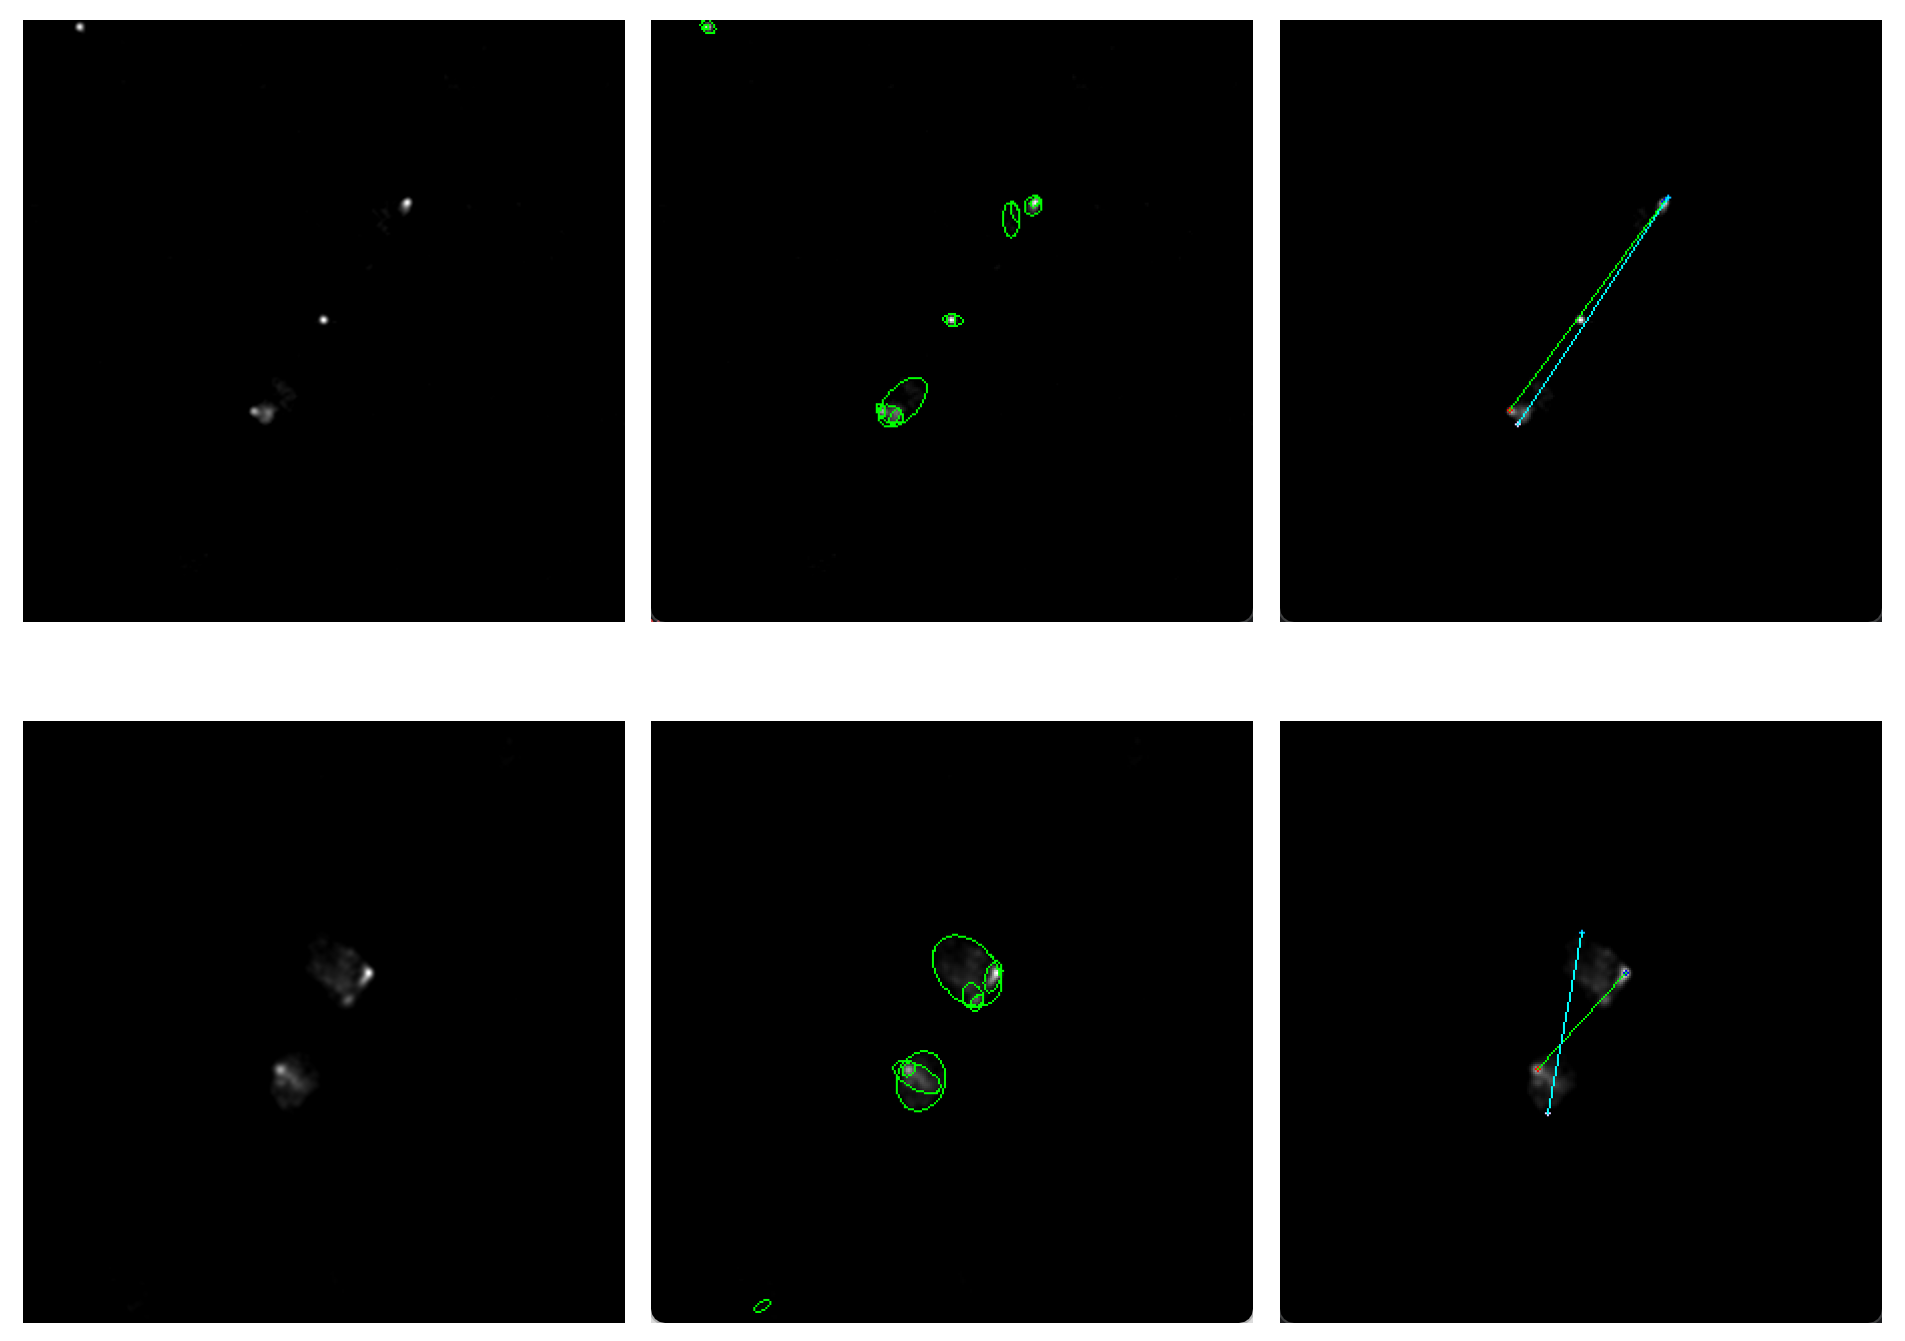
\includegraphics[width=0.9\linewidth]{Figure/Section 3/Different_rs.png}
    \caption{The first column showcases the FRII at equatorial coordinates (R.A. 155.486°, Dec. 14.725°), while the second column displays the FRII at coordinates (R.A. 148.58°, Dec. 27.267°).}
    \label{fig:Different_rs}
\end{figure}


\section{Result}\label{sec:Result}    
\subsection{The Statistical Characteristics of Geometric Parameters}\label{sec:Section4_1}

The fitted ellipses can be described with semi-major axis and axis ratio or aspect ratio, i.e., the ratio of semi-minor axis to semi-major axis.
The fraction of the sources with different aspect ratio are shown in Figure~\ref{fig:AxisRatio}.
It can be seen that the axis ratio of FRIIs are mostly less than 0.5, while FRIs distribute over larger range.

In order to investigate whether luminosity or length scale of the radio sources are related with the ellipse, Figure~\ref{fig:AxisRatioRelationship} is plotted.
As shown in the panels, there is no obvious correlation, i.e., the radio luminosity and length scale do not depend on the axis ratio. 
However, it is interesting to note that, for the cases with very small axis ratio, i.e. 0.2-0.4, only FRIIs exhibit luminosities above $10^27$ W\/Hz or  linear sizes exceeding 400 kpc. 
Additionally, there is a broad correlation between the linear size and aspect ratio for FRII sources

\begin{figure}[!htbp]
    \centering
    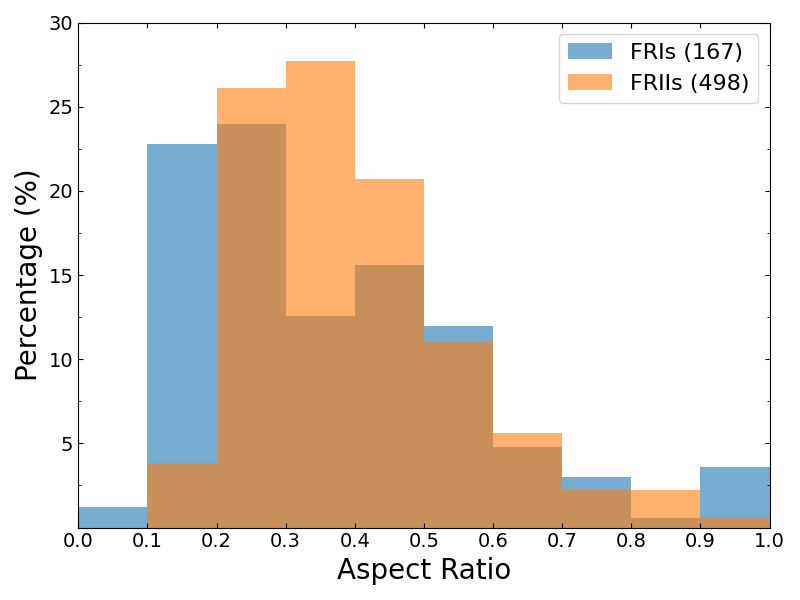
\includegraphics[width=0.9\linewidth]{Figure/Section 4/AxisRatio.png}
    \caption{Based on the elliptical structures illustrated in \autoref{fig:Figure2}, the axis-ratio distributions for FRIs and FRIIs can be statistically derived.}
    \label{fig:AxisRatio}
\end{figure}
\begin{figure*}[!htbp]
    \centering
    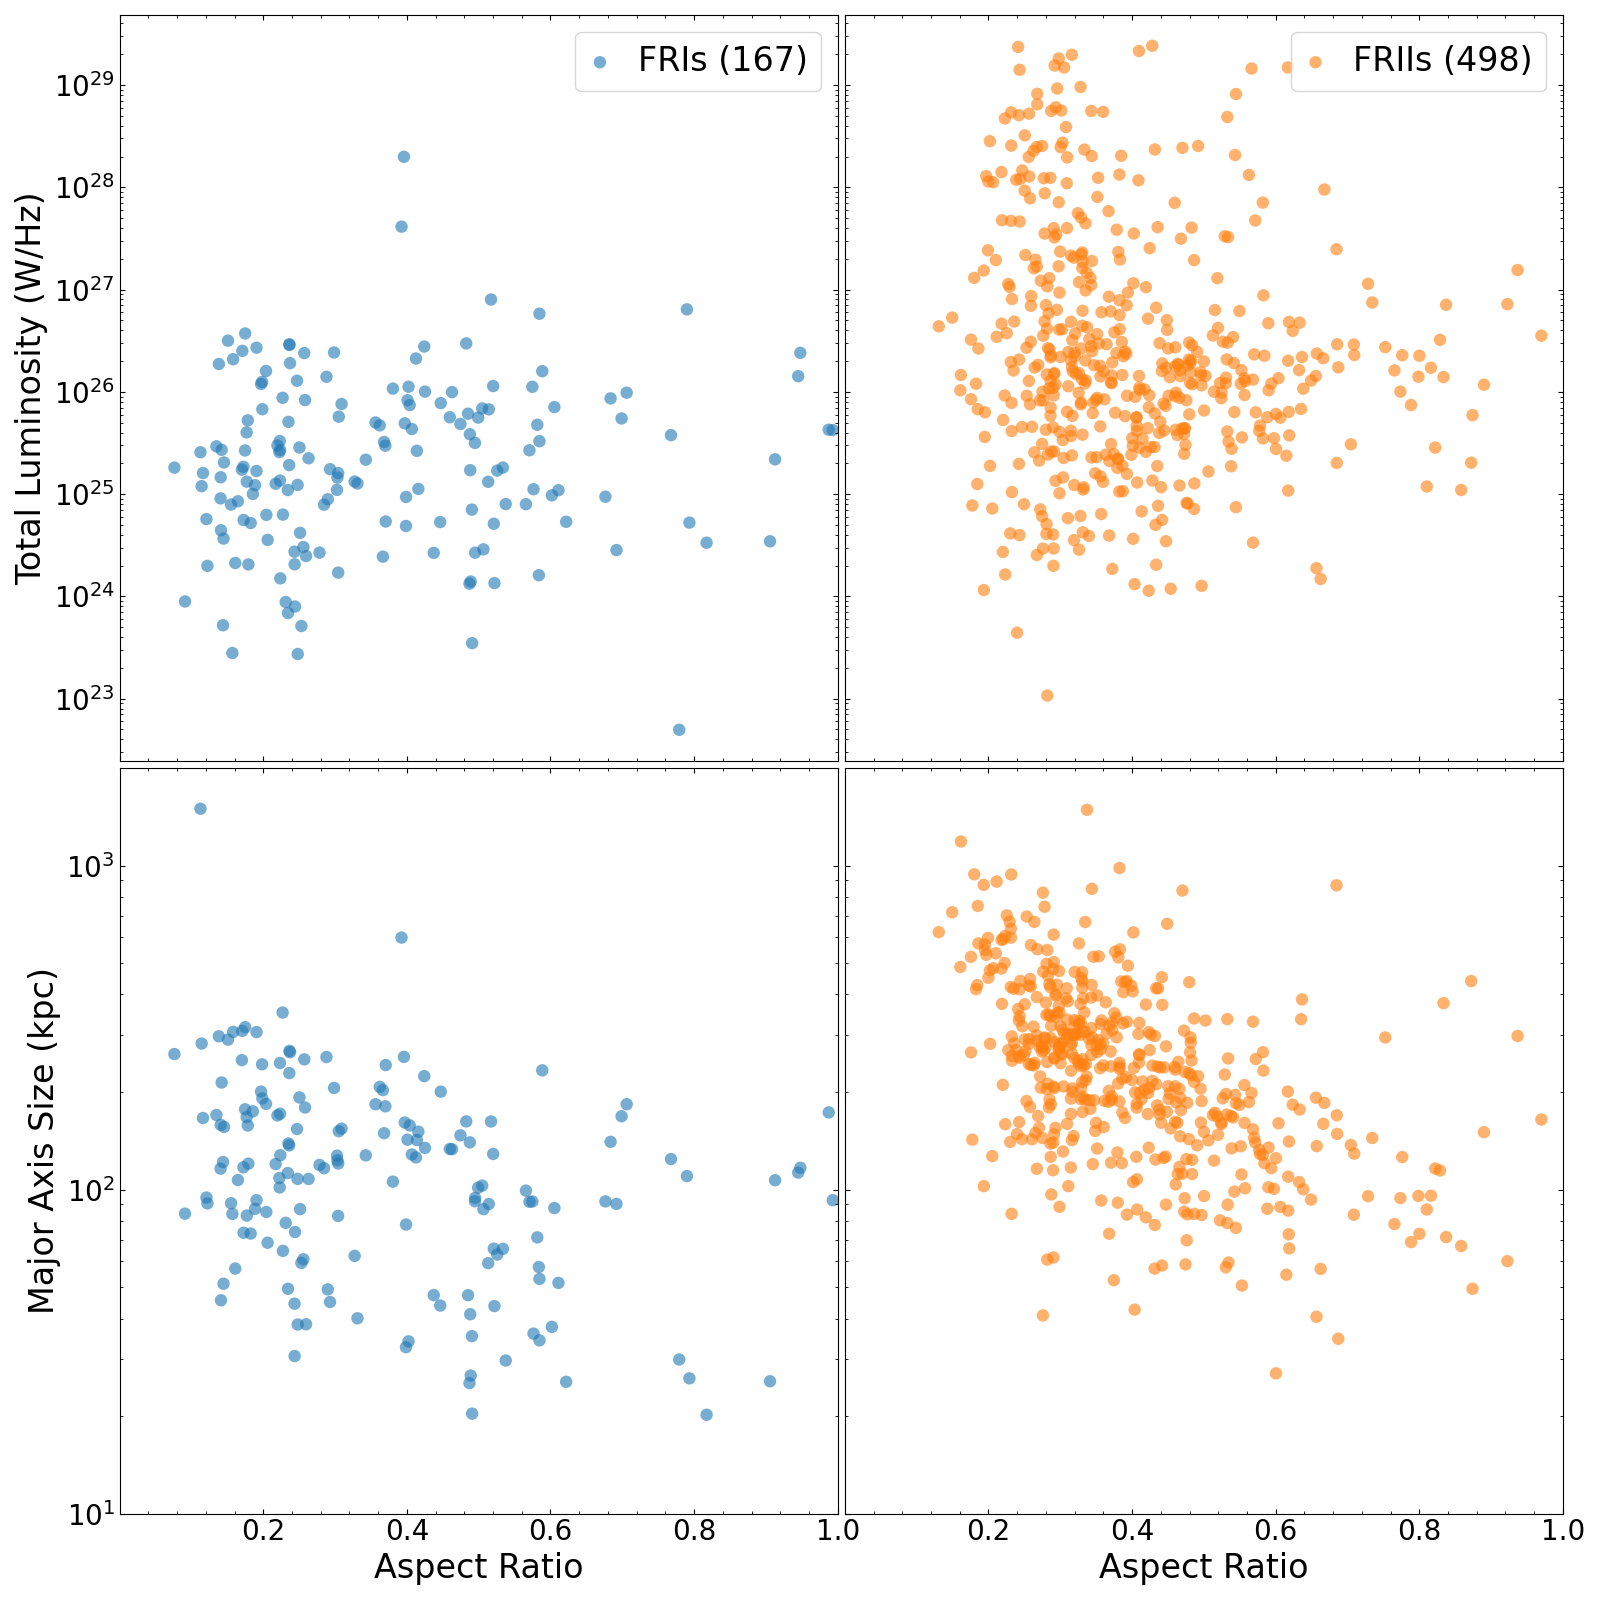
\includegraphics[width=0.8\linewidth]{Figure/Section 4/AxisRatioRelationship.png}
    \caption{Presented here are the underlying distribution characteristics of the aspect ratio relative to total luminosity and elliptical major axis size for RGs of different FR types. A distinctly offset distribution is clearly observed between the FRI-type and FRII-type populations in the figure.}
    \label{fig:AxisRatioRelationship}
\end{figure*}
\begin{figure}[!htbp]
    \centering
    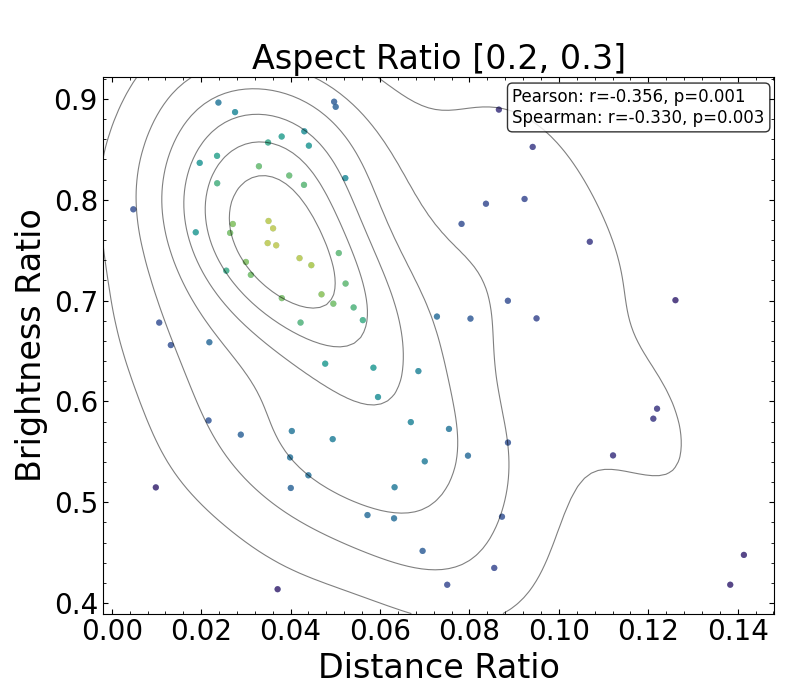
\includegraphics[width=0.8\linewidth]{Figure/Section 4/DistanceBrightnessRelationship.png}
    \caption{This figure illustrates the potential correlation between the separation of the double lobes and the brightness distribution for FRIIs within a specific range of aspect ratios. The horizontal axis represents the ratio of the double-lobe distance to the elliptical major axis size of FRIIs, while the vertical axis denotes the ratio of the radio brightness on the two sides, obtained by dividing each FRII into two parts centered on its optical counterpart. The brightness contribution from any radio lump coinciding with the optical counterpart is excluded from the calculation.}
    \label{fig:DistanceBrightnessRelationship}
\end{figure}

\begin{figure*}[!htbp]
    \centering
    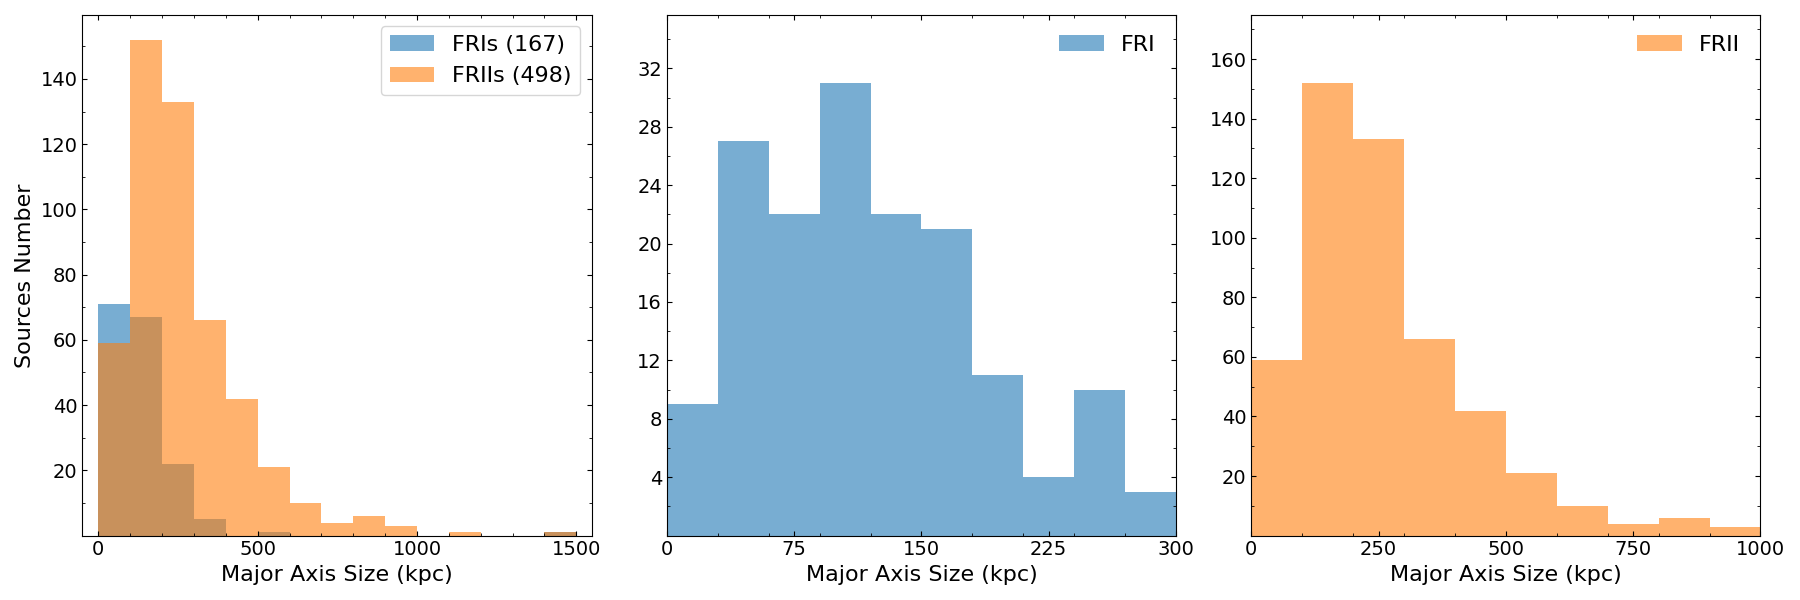
\includegraphics[width=0.9\linewidth]{Figure/Section 4/Max_Scale_Distribution.png}
    \caption{Based on the major axes of the ellipses illustrated in \autoref{fig:Figure2}, the elliptical major axis size distributions for FRIs (left panel) and FRIIs (right panel)  can be statistically derived.}
    \label{fig:Max_Scale_Distribution}
\end{figure*}


% Nodes分布特征
\subsection{The Node Structure of FRIs}\label{sec:Section4_2}

\begin{figure*}[!htbp]
    \centering
    
\includegraphics[width=0.3\linewidth]{Figure/Section 4/KnotSimple1.png}
    
\includegraphics[width=0.3\linewidth]{Figure/Section 4/KnotSimple2.png}
    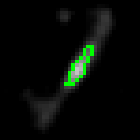
\includegraphics[width=0.3\linewidth]{Figure/Section 4/KnotSimple3.png}
    \caption{By applying the flood-filling algorithm, knots within RGs are gradually revealed and subsequently disappear as the threshold increases.}
    \label{fig:KnotSimple}
\end{figure*}

\begin{figure*}[!htbp]
    \centering
    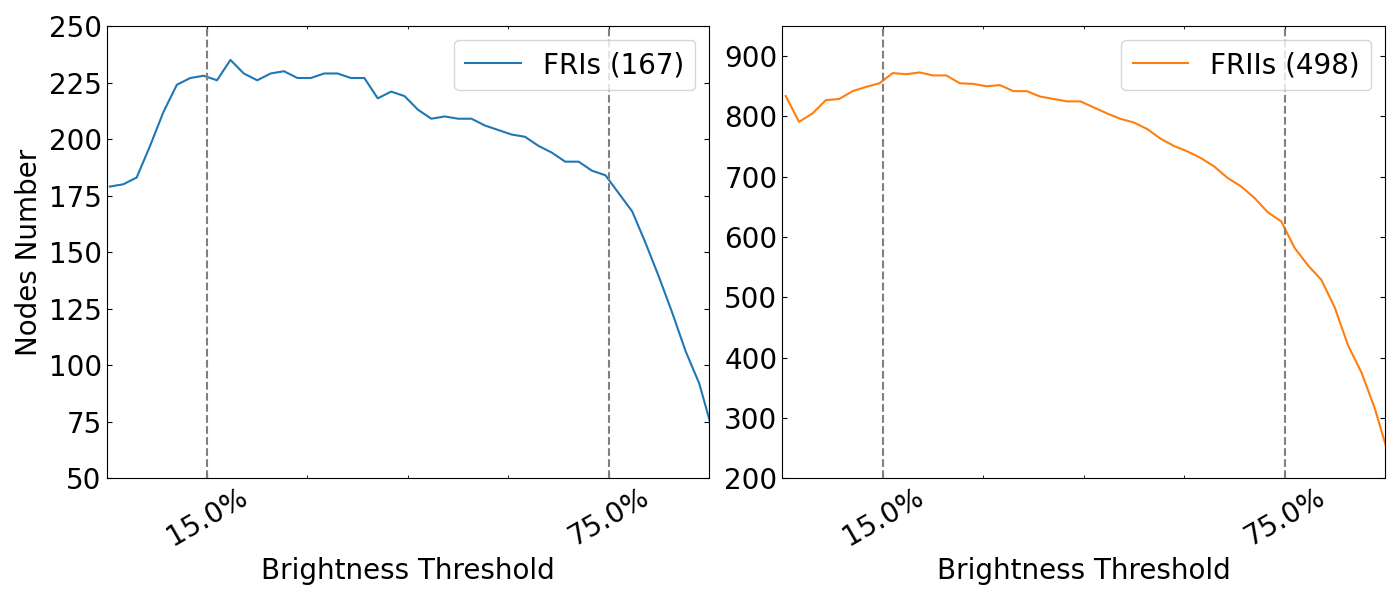
\includegraphics[width=0.9\linewidth]{Figure/Section 4/Node_Evolution.png}
    \caption{Based on the flood-filling algorithm illustrated in \autoref{fig:KnotSimple}, the total number of knots in the sample can be quantified and presented. To reduce the influence of statistical fluctuations, a threshold interval of 2\% peak brightness is adopted for the abscissa in the figure. In practice, the algorithm uses a step size of 0.5\% of the peak brightness, which may be overly fine for some faint sources. }\label{fig:Node_Evolution}
\end{figure*}
% \clearpage



\subsection{Classification Parameter $r_s$}\label{sec:Section4_3}

% \begin{figure}
%     \centering
%     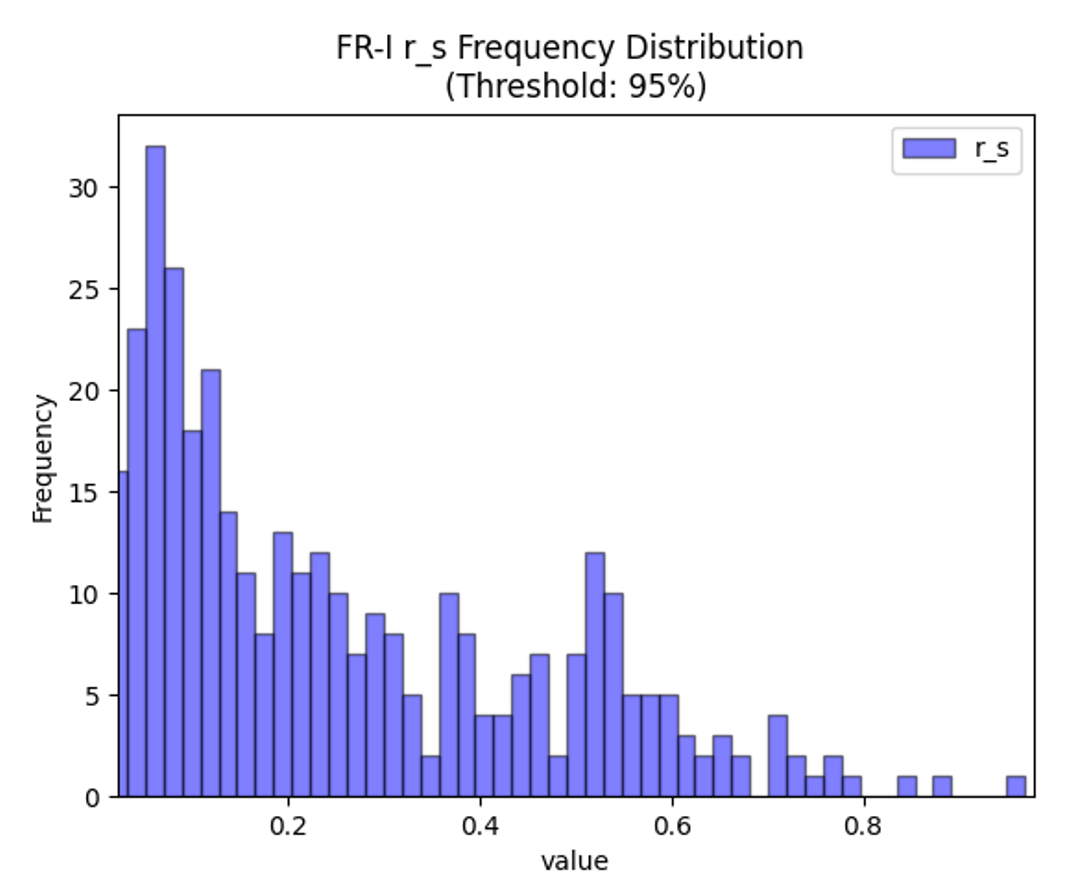
\includegraphics[width=0.9\linewidth]{Figure/Section 4/FR1_rs.png}
%     \caption{Distribution of $r_s$ values for FRIs. The horizontal axis represents the magnitude of $r_s$ values, and the vertical axis denotes the occurrence frequency of RGs corresponding to each $r_s$ value.}
%     \label{fig:11}
% \end{figure}
\begin{figure*}[!htbp]
    \centering
    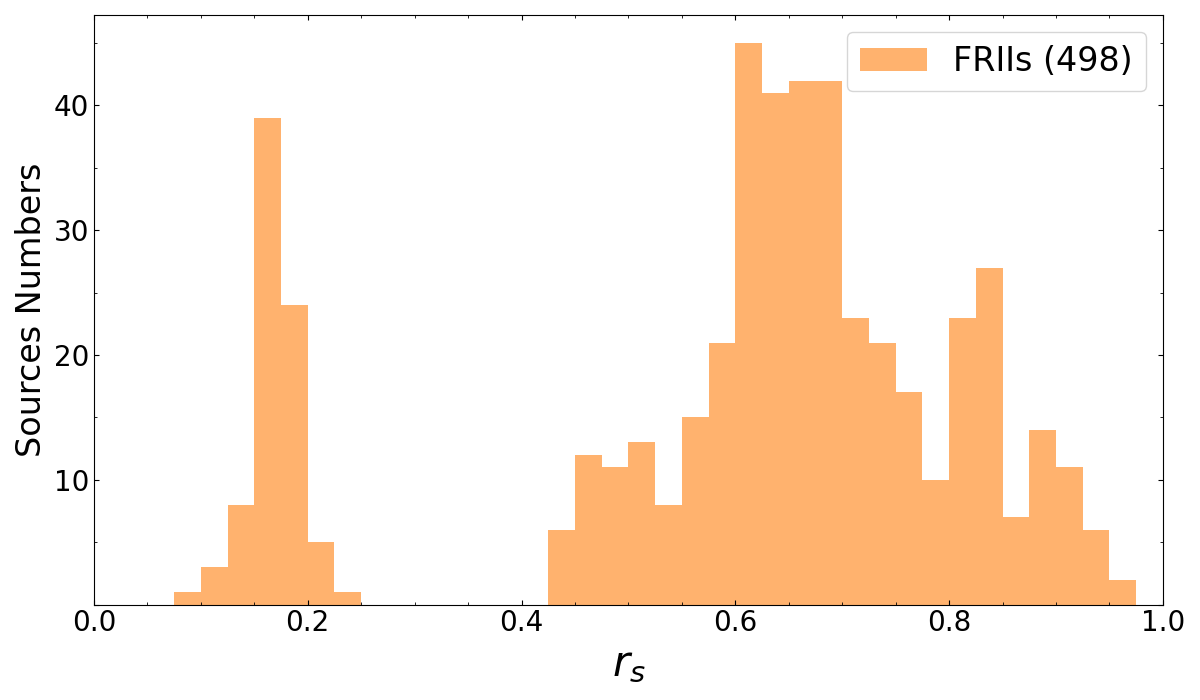
\includegraphics[width=0.45\linewidth]{Figure/Section 4/r_s_distribution0.png}
    \caption{
    Presents the distribution of $r_s$ for brightness thresholds of 95\% (blue) and 50\% (blue, completely obscured by the underlying wine red).
    }
    \label{fig:r_s_distribution0}
\end{figure*}
    % 和3D 一起绘制
    % Left Panel: Presents the distribution of $r_s$ for brightness thresholds of 90\% (orange) and 95\% (red, fully obscured by the orange). Right Panel: Presents the distribution of $r_s$ for brightness thresholds of 95\%,90\%,80\%,70\%,60\% and 50\%.



\subsection{The Feature of Central line Brightness Stacking Curve}\label{sec:Section4_4}


\begin{figure}[!htbp]
    \centering
    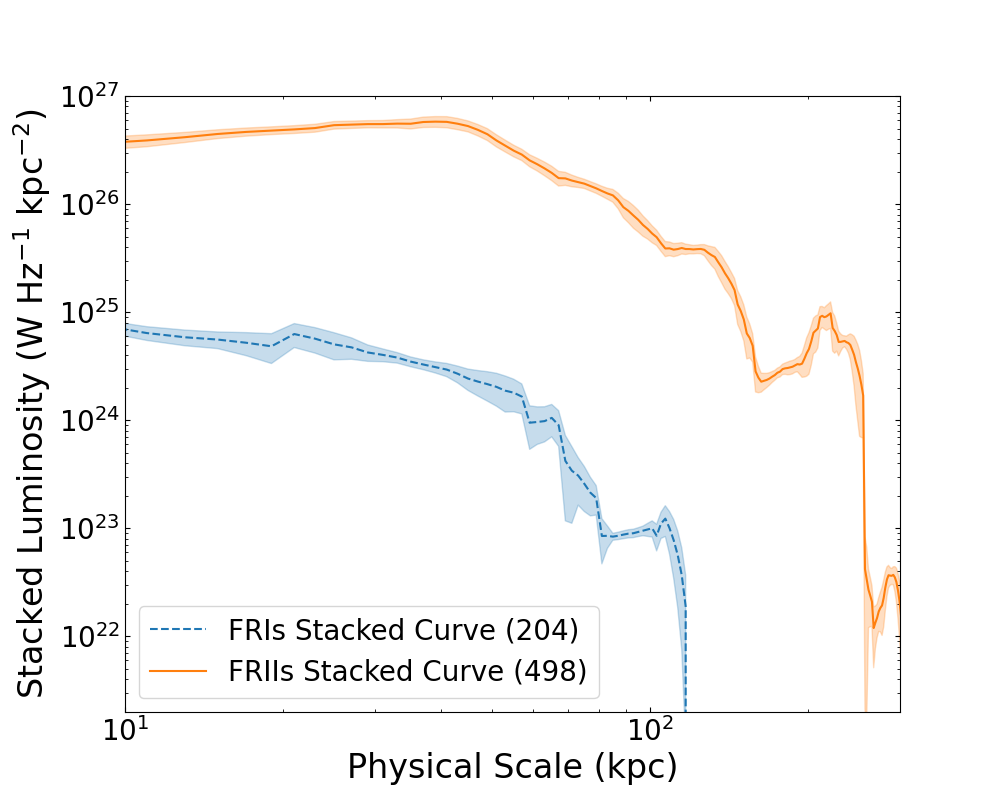
\includegraphics[width=0.9\linewidth]{Figure/Section 4/StackingCurve.png}
    \caption{Based on the flood-filling algorithm illustrated in \autoref{fig:CentralLine}, the central-line brightness stacking curve for FRIIs is presented here. In contrast to the display in the right panel of \autoref{fig:CentralLine}, each single central line of an RG is folded about its center to yield two brightness profiles, which are subsequently stacked together. This figure presents the final stacked average brightness profiles derived from 206 FRIs (blue curve) and 375 FRIIs (red curve), respectively, where the shaded region denotes the uncertainty in the brightness distribution. }
    \label{fig:13}
\end{figure}


% 由于之前提到不再讨论倾角问题，所以伸长参数这一块还是不写了
    % % 伸长参数
    % \subsection{The Distribution of Elongation Parameter}\label{sec:Section4_5}
    
    
    % \begin{figure*}
    %     \centering
    %     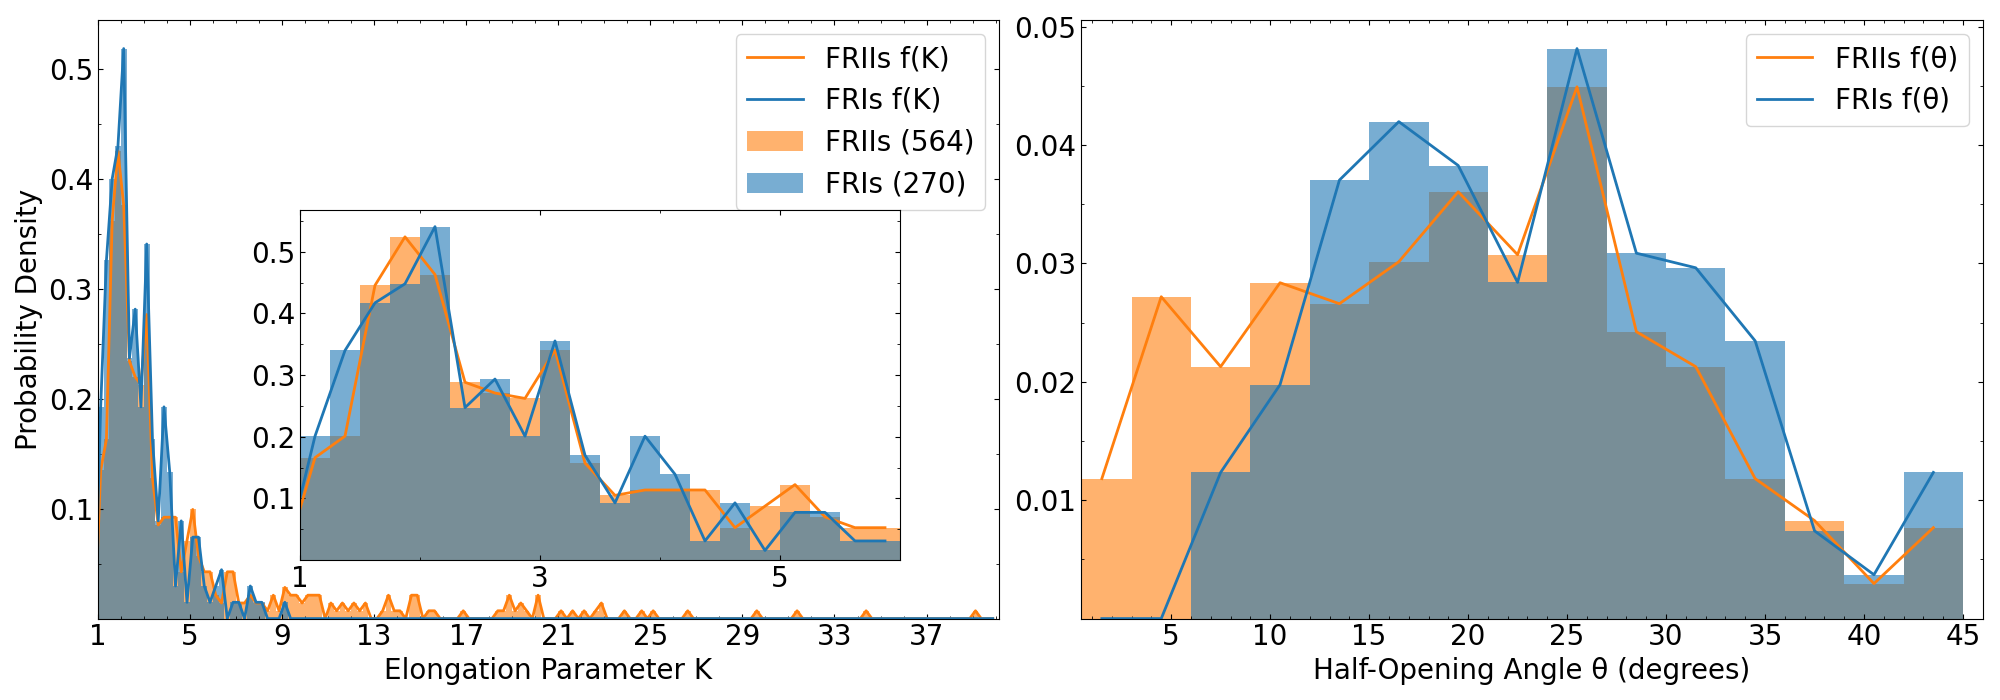
\includegraphics[width=0.9\linewidth]{Figure/Section 4/ProbabilityDensity.png}
    %     \caption{Left Panel: Probability density distribution of the elongation parameter K; The horizontal axis represents K, and the vertical axis denotes the probability density of K; Histogram bins for K are set at intervals of 0.25, with the corresponding curve $f(K)$ representing the probability density function of K; Red and blue colors correspond to FRIs and FRIIs, respectively. Right Panel: Probability density distribution of the half-opening angles ($\theta$) of RGs estimated using K; The horizontal axis represents the $\theta$, and the vertical axis denotes the probability density of the $\theta$; Histogram bins for the $\theta$ are set at intervals of $3^\circ$ , with the corresponding curve $f(\theta)$ representing the probability density function of the $\theta$.}
    %     \label{fig:14}
    % \end{figure*}
    % % \clearpage


\section{Discussion}\label{sec:Discussion}

\begin{figure}
    \centering
    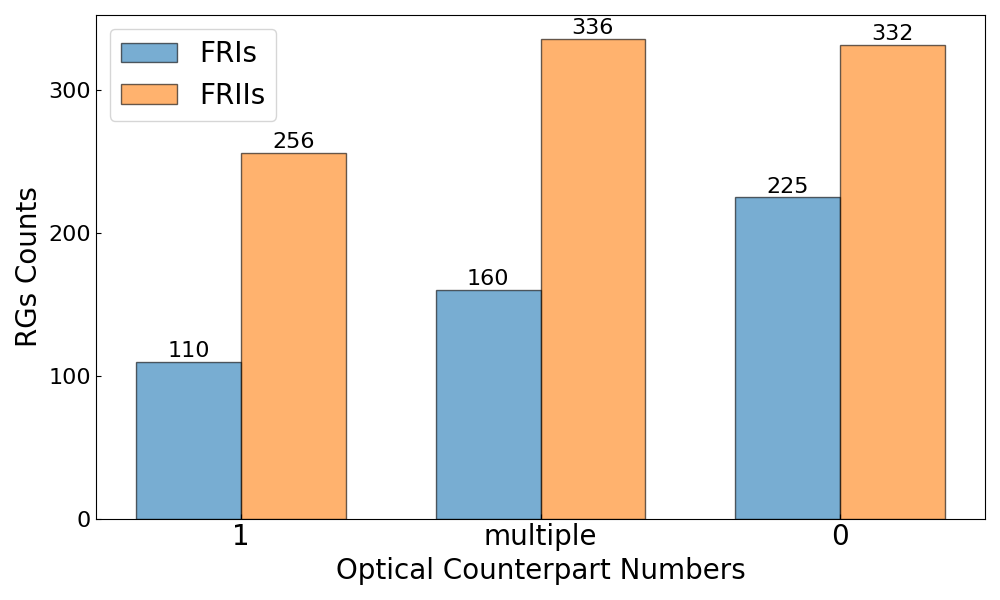
\includegraphics[width=0.9\linewidth]{Figure/Section 5/OpticalCounterpartCountDistributions.png}
    \caption{This figure illustrates the distribution of RGs during the search for their optical counterparts. The two colored labels correspond to FRI/FRII-type RGs, respectively. The horizontal axis represents the number of optical counterparts detected for each RG: optical counterparts with a detection count of 1 are relatively more reliable than those with a count of "multiple", and RGs with an optical counterpart count of 0 will be excluded from our subsequent analysis. The vertical axis denotes the number of RGs.}
    \label{fig:OpticalCounterpartCountDistributions}
\end{figure}
\subsection{The Deviations in Procedure}\label{sec:Section5_1}


\subsection{Similar Mechanism of Morphological Evolution?}\label{sec:Section5_2}




\bibliographystyle{aa}
\bibliography{BibDir/Introduction,BibDir/Data,BibDir/Method,BibDir/Discussion}
\begin{appendix}
\section{Alternative thread identification}\label{app:Alt} 




\end{appendix}






\end{document}

